% ============================================================================
% SPoS-MSC v4 SENSITIVITY-COMPLETE REVISION
% - Uses v3 as the predecessor self-logging model and v4 as the public
%   sensitivity-enabled executable model.
% - Reports 700 native Q1--Q7 scenario replications and 2,400 native local
%   OFAT sensitivity replications.
% - Treats the Python/FastAPI artefact as a reference runtime emulator.
% - Makes no causal-ablation, public-network TPS, or shard-scale-out claim.
% - Author-supplied CRediT, funding, competing-interest, ORCID, and archival
%   DOI details require confirmation before submission.
% ============================================================================
% Elsevier CAS single-column format (cas-sc.cls)
\documentclass[a4paper,fleqn]{cas-sc}

% Packages (keep only what you use)
\usepackage{amsmath,amssymb,amsfonts}
\usepackage{graphicx}
\usepackage{xcolor}
\usepackage{booktabs}
\usepackage{array}
\usepackage{tabularx}
\usepackage{multirow}
\usepackage{makecell}
\usepackage{algorithm}
\usepackage{algorithmic}
\usepackage{url}
\definecolor{journalblue}{RGB}{0,118,168}
\hypersetup{
  hypertexnames=false,
  colorlinks=true,
  linkcolor=journalblue,
  citecolor=journalblue,
  urlcolor=journalblue,
  pdftitle={Executable Modelling of a Sharded Mobile Smart-Contract Lifecycle with Incentive-Aware Proof-of-Stake Governance},
  pdfauthor={Vipin Deval; Vimal Dwivedi; Alex Norta; Dirk Draheim},
  pdfkeywords={blockchain simulation; Coloured Petri Nets; mobile smart contracts; Proof-of-Stake; sharding; sensitivity analysis}
}

% Submission-safe typography: rely on the Elsevier CAS class defaults.
\usepackage{microtype}
\usepackage{enumitem}
\setlist[itemize]{leftmargin=1.45em,itemsep=1pt,topsep=3pt,parsep=0pt,partopsep=0pt}
\setlist[enumerate]{leftmargin=1.65em,itemsep=1pt,topsep=3pt,parsep=0pt,partopsep=0pt}

% Float placement helpers
\usepackage{placeins}
\usepackage{float}
\usepackage{flafter}
\makeatletter
\def\fps@figure{htbp}
\def\fps@table{htbp}
\makeatother

% Improve float packing to reduce large blank areas caused by deferred floats
\setcounter{topnumber}{2}
\setcounter{bottomnumber}{1}
\setcounter{totalnumber}{3}
\renewcommand{\topfraction}{0.95}
\renewcommand{\bottomfraction}{0.8}
\renewcommand{\textfraction}{0.05}
\renewcommand{\floatpagefraction}{0.85}
\renewcommand{\dbltopfraction}{0.95}
\renewcommand{\dblfloatpagefraction}{0.85}

% Bibliography/citation setup (Elsevier CAS uses natbib)
\usepackage[numbers]{natbib}
\setcitestyle{numbers,square,comma,sort&compress}

\newcommand{\model}{SPoS-MSC}

% Suppress the CAS front-matter ORCID note when no ORCID metadata is supplied.
% The original note appears automatically as soon as one or more authors receive
% an `orcid=...` key.
\ExplSyntaxOn
\cs_new_eq:NN \spos_original_printorcid: \printorcid
\RenewDocumentCommand \printorcid { }
  { \seq_if_empty:NF \g_stm_orcid_seq { \spos_original_printorcid: } }
\ExplSyntaxOff

\begin{document}
\let\WriteBookmarks\relax

\shorttitle{Executable Modelling of a Sharded MSC Lifecycle with iPoS Governance}
\shortauthors{Deval et~al.}

\title[mode=title]{Executable Modelling of a Sharded Mobile Smart-Contract Lifecycle with Incentive-Aware Proof-of-Stake Governance}
\author[aff1,aff2]{Vipin Deval}\corref{cor1}
\ead{vipin.deval@taltech.ee}

\author[aff3]{Vimal Dwivedi}

\author[aff4,aff5]{Alex Norta}

\author[aff1]{Dirk Draheim}

\cortext[cor1]{Corresponding author}

\affiliation[aff1]{organization={Information Systems Group, Tallinn University of Technology},city={Tallinn},country={Estonia}}
\affiliation[aff2]{organization={Krishna Institute of Engineering \& Technology},city={Ghaziabad (Delhi-NCR)},country={India}}
\affiliation[aff3]{organization={Intelligent System Research Center, Center for Legal Technology, Ulster University},country={United Kingdom}}
\affiliation[aff4]{organization={Tallinn University},city={Tallinn},country={Estonia}}
\affiliation[aff5]{organization={University of Pretoria},city={Pretoria},country={South Africa}}

\begin{abstract}
Mobile smart-contract systems must coordinate resource-aware request preparation,
sharded execution, validator governance, quorum finality, root-chain commitment,
receipt delivery, incentives, and auditable evidence. Existing sharding
protocols, Proof-of-Stake (PoS) studies, and formal blockchain models commonly
examine these concerns separately, leaving their cross-layer interactions
insufficiently represented. This paper presents SPoS-MSC, a
requirements-traceable hierarchical Coloured Petri Net (CPN) model of a mobile
smart-contract lifecycle governed by incentive-aware PoS, together with a
separate reference runtime emulator. The public v4 executable contains four
execution domains and eight functional stages covering mobile request
admission, adaptive shard routing, owner-aware validator scoring, committee
formation and recovery, smart-contract execution and proof generation,
distinct-member quorum finality, root-chain commitment, mobile receipt
delivery, incentive feedback, decentralisation measurement, and explicit run
termination. Across seven scenarios and 700 native CPN Tools replications, the
evaluation covers 19,600 submitted transactions and produces 18,767 finality
certificates, 18,767 root commitments, and 18,187 mobile receipts.
Transaction-weighted finality and receipt success equal 95.75\% and 92.79\%,
respectively. A further 2,400-run local one-factor-at-a-time sensitivity
analysis shows strong responses to workload, cross-shard demand, request
disconnection, receipt delivery, committee configuration, and load threshold.
Most notably, increasing the mobile-fitness threshold from 35 to 65 reduces the
eligible validator set from six to three and finality/receipt success from
100\% to 75\%, exposing a threshold-dependent
security--availability--decentralisation trade-off. All 700 scenario
replications and 2,400 sensitivity replications terminate explicitly, and the
recorded outputs satisfy the lifecycle-ordering and terminal-accounting
invariants. Poor connectivity remains the principal liveness constraint;
cross-shard and hot-shard workloads mainly increase latency, load dispersion,
and reconfiguration; and risk-aware filtering with committee recovery preserves
completion while increasing reward concentration. The contribution is a
reproducible cross-layer modelling and evidence framework rather than a claim
of superior public-network performance.
\end{abstract}

\begin{keywords}
blockchain simulation \sep formal modelling \sep mobile smart contracts \sep
sensitivity analysis \sep Proof-of-Stake governance \sep sharded blockchains
\sep validator decentralisation
\end{keywords}

\maketitle
\hypersetup{
  pdfauthor={Vipin Deval; Vimal Dwivedi; Alex Norta; Dirk Draheim},
  pdftitle={Executable Modelling of a Sharded Mobile Smart-Contract Lifecycle with Incentive-Aware Proof-of-Stake Governance},
  pdfkeywords={blockchain simulation; Coloured Petri Nets; mobile smart contracts; Proof-of-Stake; sharding; sensitivity analysis}
}
\normalsize

\section{Introduction}
\label{sec:introduction}

Mobile participation changes the boundary of smart-contract execution. A transaction is created and signed on a resource-constrained device, prepared with support from an edge or access component, assigned to a shard, validated by a committee, committed through a root-level decision, and returned to the user as compact finality evidence. In this paper, the term \emph{mobile smart contract} (MSC) is used operationally to describe the complete mobile smart contract lifecycle. It does not imply that every stage is executed by the same mobile device. Instead, participation is role- and resource-dependent: a device may create transactions, monitor contract state, or verify receipts, while a resource-qualified mobile or edge-assisted validator may also participate in shard-block validation, proof generation, or root-block validation. The lifecycle considered here therefore extends from mobile request preparation to shard processing, finality, root-chain commitment, receipt generation, and auditability. 

The first challenge in this lifecycle is scalability. Processing every mobile-originated request through one globally replicated execution path would preserve the conventional blockchain bottleneck while adding the cost of intermittent connectivity, edge preparation, compact verification, and receipt delivery~\cite{Boughdiri2025,LIU2024,cortes2025impact,HEWA2021survey}. Layer-2 execution, state channels~\cite{Liu2025SharHSC,Negka2021StateChannels}, off-chain computation~\cite{Tan2025OffChain,Cai2022Offchain}, DAG-based ledgers~\cite{Wang2023DAG,Li2023DAG}, and execution-layer parallelism~\cite{Chen2023Parallel} address related scalability problems. This study focuses on sharding because its research problem concerns the interaction among transaction placement, shard-local execution, cross-shard evidence, validator committees, and root-level commitment. Existing protocols such as ELASTICO~\cite{Luu2016}, OmniLedger~\cite{Kokoris-Kogias2018}, RapidChain~\cite{Zamani2018a}, and Chainspace~\cite{Al-Bassam} demonstrate that shard formation and parallel processing can increase blockchain capacity, while allocation mechanisms such as BrokerChain~\cite{Huang2022Brokerchain} and TxAllo~\cite{Zhang2023TxAllo} show that transaction placement and workload imbalance strongly influence performance. These systems provide important scalability foundations, but they generally model infrastructure-oriented transaction streams rather than an end-to-end mobile lifecycle in which request admission, device suitability, proof evidence, and receipt delivery are explicit protocol states.

Once execution is distributed across shards, however, scalability becomes inseparable from consensus governance. Each shard requires validators that can process its transactions, reach finality, and produce evidence that can be committed and returned to mobile users. Proof-of-Stake (PoS) is attractive for this purpose because it replaces energy-intensive mining with economically bonded validation. Yet raw stake-proportional selection may concentrate consensus duties and rewards among already dominant validators
or owners. Repeated selection, reward accumulation, restaking, and delegation can reinforce this concentration over time
\cite{Li2023Rewarddistribution,LEPORATI2024,Tang2024,
Erdem2025Proof,Gersbach2026}. The issue is more complex in a mobile setting, where stake is not a sufficient measure of suitability. A high-stake validator may be unavailable, resource-constrained, or exposed to elevated attack risk, whereas a lower-stake validator may be reliable and mobile-suitable but rarely selected. Shard governance must therefore account for ownership, effective stake, mobile fitness, risk, committee composition, finality contribution, rewards, penalties, and decentralisation together.

This interaction creates the central modelling problem of the paper.
Sharding research explains how transaction and state workloads can be
partitioned, while PoS and Byzantine fault-tolerant (BFT) protocols explain how validators can be selected and how committees can reach finality. Studies of decentralisation measure inequality, concentration, and control thresholds through indicators such as the Gini coefficient, Herfindahl--Hirschman Index (HHI), and Nakamoto coefficient
\cite{MENG2023Gini,motepalli2025pos,nakai2024}.
Among the closest methodological studies, blockchain-sharding emulators provide controlled measurements of throughput, latency, workload distribution, and cross-shard activity, whereas CPN-based blockchain studies formalise individual protocol lifecycles and their state-transition dependencies~\cite{Huang2025BlockEmulator,Sujatanagarjuna2021BlockVoke}. Neither category connects mobile-resource-aware lifecycle execution, owner-aware PoS governance, root-commitment and receipt evidence, reward/slashing feedback, load reconfiguration, and decentralisation monitoring in one requirements-traceable executable model. This separation is important because an improvement at one layer may produce a cost at another: a routing policy may increase throughput but also increase receipt latency, while strict validator filtering may improve committee safety but concentrate work and rewards among fewer participants.

This paper addresses that problem through SPoS-MSC, an integrated modelling and simulation framework for a sharded mobile smart-contract lifecycle with incentive-aware PoS governance. The lifecycle component represents mobile request preparation, shard routing, validation, committee-controlled finality, root-chain commitment, and receipt generation; the governance component represents owner-aware stake treatment, mobile- and risk-based eligibility, committee selection and recovery, rewards, slashing, and decentralisation feedback. The two components meet at committee-controlled
finality: governance determines which committee may finalise a routed
transaction, while the resulting finality and receipt evidence drive
commitment, incentives, and evaluation outputs. The novelty lies in this executable cross-layer integration and its traceability from requirements to model state and measured evidence.

A Qtum\footnote{https://qtum.org/}-inspired running case gives the model a concrete transaction,
execution, and verification context. Qtum is selected not because it is assumed to be superior to Ethereum~\cite{ROSABILBAO2023Ethereum}, Cardano~\cite{Niya2023Cardano}, Polkadot~\cite{Abbas2022Polkadot}, Avalanche~\cite{Tanana2019Avalanche}, or other PoS platforms, but because one platform combines the four abstractions needed by the running case: an unspent transaction output (UTXO)-oriented transaction foundation, account abstraction for smart-contract execution, PoS operation, and lightweight verification \cite{Chen2020,dai2017smart}. This combination provides a
coherent setting for mobile request signing, stake-backed validation, and compact receipt evidence. The proposed sharding, committee governance, root-commitment abstraction, and reported measurements belong to SPoS-MSC; they are not modifications of, or observations from, the production Qtum network.

The study follows a requirements-to-model-to-evidence process. First,
Agent-Oriented Modelling (AOM) is used to identify functional goals, quality goals, roles, responsibilities, and traceability obligations
\cite{Sterling2009,yu2002}. Second, these requirements are formalised as a hierarchical Coloured Petri Net (CPN) model. Typed tokens represent mobile transactions, validators, ownership-aware scores, committees, shard loads, finality certificates, root commitments, receipts, rewards, slashing records, and evaluation evidence. Guards and arc inscriptions define transaction admission, routing, validator eligibility, committee formation, finality, receipt generation, feedback, and reconfiguration. The CPN model formalises typed protocol states and guarded transition dependencies and supports structural safety arguments for routing integrity, committee-dependent finality, quarantine exclusion, receipt-after-commitment, and overload observability. Third, 700 repeated native CPN scenario runs provide bounded evidence about composite model behaviour; they do not constitute exhaustive state-space verification. Fourth, a local sensitivity study comprising 2,400 native CPN replications evaluates eight executable controls at low, default, and high levels, separating composite scenario behaviour from local parameter robustness. A separate reference runtime emulator then provides a secondary engineering check under analogous scenario families; it does not constitute a distributed blockchain implementation. The CPN layer therefore supplies the primary formal, scenario, and sensitivity evidence, whereas the runtime emulator supplies secondary implementation-level trend evidence.


The study is guided by the following main research question:
\begin{quote}
\emph{How can an incentivised PoS mechanism be integrated with a sharded MSC lifecycle so that mobile suitability, receipt-level finality, validator decentralisation, and scalability-related stress can be represented and evaluated in one executable model?}
\end{quote}

The question is refined into three sub-questions:

\begin{itemize}
    \item \textbf{RQ1:} What functional, quality, stakeholder, security, incentive, and evidence requirements define the integrated mobile-smart-contract lifecycle and its PoS governance?

    \item \textbf{RQ2:} What CPN structure and formal semantics realise these requirements from mobile request preparation and shard routing to committee-controlled finality, root-chain commitment, receipt generation, and reward/slashing feedback?

    \item \textbf{RQ3:} What evidence do native CPN scenario simulations, local parameter-sensitivity analysis, and a reference runtime emulator provide about lifecycle completion, scalability-related stress, resilience, incentive behaviour, and validator decentralisation?
\end{itemize}

The study therefore develops four linked outputs. First, it defines an integrated lifecycle-governance abstraction for mobile smart contracts. Second, it provides an executable CPN specification that connects AOM-derived requirements to protocol state, transition semantics, and structural safety properties. Third, it evaluates the resulting model through 700 native Q1--Q7 scenario replications and 2,400 native local OFAT replications, using lifecycle, load, resilience, incentive, and decentralisation metrics. Fourth, it applies a separately scoped reference runtime emulator under analogous scenario labels to examine cross-layer trend consistency. Conclusions about performance derive from the controlled SPoS-MSC experiments; values reported by external systems provide metric-level context only.

The remainder of the paper is organised as follows.
Section~\ref{sec:background} reviews the foundations and related work on mobile smart contracts, sharding, PoS governance, decentralisation, and blockchain modelling, and introduces the running case and research gap. Section~\ref{sec:aom} derives the AOM goal model and traceable requirements. Section~\ref{sec:framework} presents the integrated protocol and its CPN formalisation. Section~\ref{sec:methodology} defines the native Q1--Q7 experiment, the local one-factor-at-a-time (OFAT) sensitivity design, the statistical procedures, and the reference-runtime boundary. Section~\ref{sec:results} reports scenario behaviour, parameter sensitivity, cross-layer trend agreement, and the integrated answer to RQ3.

\section{Background and Related Work}
\label{sec:background}

This section reviews the literature needed to position SPoS-MSC as a modelling and simulation artefact. The discussion follows the same logic as the introduction. First, mobile smart contracts require lifecycle-level evidence rather than only transaction inclusion. Second, sharding improves scalability but introduces routing, cross-shard, and load-balance issues. Third, shard execution requires validator committees, so PoS governance becomes part of the scalability problem. Fourth, the resulting lifecycle-consensus interaction must be represented in an executable model that supports simulation, monitoring, and validation.

\subsection{Mobile Smart Contracts and Lifecycle Evidence}\label{subsec:msc_constraints}

A mobile smart-contract lifecycle starts before a transaction enters the blockchain mempool and continues after block inclusion. A mobile user must create and sign a request, submit it through an access or edge layer, receive compact evidence, and verify that the request reached a final state. Lightweight verification such as Simplified Payment Verification (SPV) reduces storage and computation by checking compact inclusion evidence rather than the full ledger~\cite{Qin2019SPV}. In MSCs, however, the evidence required by the user may cover more than payment inclusion. A mobile participant may need to know that the transaction reaches the correct shard, enters a shard block, passes proof-backed validation, receives root- or main-chain acceptance, and terminates through a verifiable receipt.

This broader evidence requirement makes MSC different from ordinary client-side blockchain interaction. The mobile device is not assumed to execute the complete smart contract or maintain the full chain. Instead, it participates in a lifecycle that must remain feasible under battery, CPU, wallet, storage, network, and availability constraints. This motivates a modelling view in which transaction creation, edge packaging, shard routing, proof-backed validation, receipt finality, and evidence logging are represented as connected lifecycle states. Once the lifecycle includes shard assignment and proof/receipt evidence, scalability mechanisms such as sharding become relevant, but they must be interpreted through mobile feasibility rather than throughput alone.

\subsection{Blockchain Sharding, Cross-Shard Processing, and Workload Allocation}\label{subsec:sharding}

Sharding improves scalability by allowing shards to process subsets of transactions in parallel. Infrastructure-oriented protocols such as ELASTICO, OmniLedger, and RapidChain demonstrate that shard formation and parallel processing can increase throughput under suitable assumptions~\cite{Luu2016,Kokoris-Kogias2018,Zamani2018a}. Smart-contract sharding systems such as Chainspace move this idea closer to programmable execution by supporting cross-shard commitment~\cite{Al-Bassam}. These systems are important foundations for SPoS-MSC because they show how ledger processing and smart-contract state can be distributed across smaller execution groups.

However, these protocols mainly assume infrastructure-grade validators and do not treat mobile-resource feasibility as a lifecycle-level condition. In particular, they usually treat workload as a transaction stream rather than as a mobile-originated smart-contract lifecycle with request admission, edge assistance, proof-backed validation, and receipt-stage confirmation. This distinction matters because a shard may process transactions efficiently while still failing to provide evidence that a mobile participant can verify or use. Therefore, sharding alone is not sufficient for MSC execution; the shard-routing and cross-shard mechanisms must be connected to receipt finality and mobile-suitable validator participation.

Recent work has also shifted attention from shard formation to workload placement and cross-shard reduction. TxAllo formulates dynamic transaction allocation and reports that the cross-shard ratio can be substantially reduced compared with hash-based allocation~\cite{Zhang2023TxAllo}. BrokerChain and related work treat hot shards and state placement as central scalability problems~\cite{Huang2022Brokerchain}. LARCH introduces latency-aware consistent hashing to reduce communication delay and improve throughput relative to hashing baselines~\cite{jorika2026larch}. These studies validate the metrics used later in this paper, including throughput, receipt latency, cross-shard ratio, shard-load imbalance, and reconfiguration pressure. Nevertheless, their primary concern is allocation efficiency, not the combined modelling of mobile lifecycle evidence, owner-aware PoS committees, and reward/decentralisation feedback.

\subsection{Proof-of-Stake, Incentives, and Validator Oligopoly}\label{subsec:pos_oligopoly}

Because sharded MSC execution depends on validators or committees at each shard, scalability cannot be separated from consensus governance. PoS is attractive in this context because it replaces energy-intensive mining with economically bonded validation. Secure PoS protocol families such as Ouroboros provide formal foundations for stake-based consensus~\cite{Kiayias2017}; Algorand motivates VRF-based committee selection~\cite{Chen2019b}; Ethereum-style PoS motivates validator duties, rewards, penalties, and slashing~\cite{pititto2022gasper}; and BFT protocols such as HotStuff motivate quorum-based finality~\cite{yin2019hotstuff}. These mechanisms provide essential building blocks for scalable and accountable committee operation.

The limitation is that conventional stake-proportional PoS can concentrate consensus influence. High-stake validators or owners may receive more duties, collect more rewards, and increase their future selection probability. This creates a possible staking oligopoly~\cite{Liu2023Oligopoly,deval2019}. Recent decentralisation studies, therefore, use the Gini coefficient, HHI, Nakamoto coefficient, and related measures to quantify inequality, concentration, and control thresholds~\cite{MENG2023Gini,motepalli2025pos,nakai2024}. Nonlinear weighting functions, such as square-root and logarithmic transformations, have also been proposed to reduce the marginal influence of large stakes.

For MSCs, however, concentration is not only an economic issue. Validator suitability also depends on mobile fitness, connectivity, availability, risk, and ownership structure. A high-stake validator may be unsuitable for time-critical shard finality, while a lower-stake validator may be honest and mobile-suitable but disadvantaged by raw stake weighting. Thus, an MSC-oriented PoS mechanism must jointly represent stake, ownership, mobile fitness, attack evidence, committee selection, finality, rewards, slashing, and decentralisation metrics. This requirement motivates the SPoS layer in the proposed SPoS-MSC model.

\subsection{Formal Modelling and Simulation of Blockchain Mechanisms}\label{subsec:formal_simulation}

The preceding subsections show that SPoS-MSC is not only a protocol design problem but also a modelling problem. The system contains concurrent token flows: mobile requests are created, routed, and finalised; validators are scored, filtered, and assigned to committees; receipts and rewards are generated; and metrics are recorded. Informal diagrams cannot fully expose reachability, enabledness, boundedness, dead markings, guard satisfaction, or the connection between lifecycle requirements and output evidence.

CPN Tools is suitable for this task because it combines typed tokens, guarded transitions, hierarchy, and executable simulation~\cite{Jensen2007}. In a blockchain context, CPN Tools can represent validators, transactions, committees, certificates, receipts, rewards, and metric tokens while preserving formal transition semantics. Other modelling and simulation tools are also relevant. Blockchain emulators such as BlockEmulator support experimental evaluation of sharding mechanisms using metrics such as throughput, confirmation latency, cross-shard transaction ratio, queue state, and workload distribution~\cite{Huang2025BlockEmulator}. Discrete-event simulation frameworks for sharded blockchains similarly emphasize controlled workload generation and performance measurement~\cite{wainer2017discrete}. These works support the methodological position of this paper: an integrated lifecycle-consensus proposal should be evaluated using traceable model states, repeated scenarios, and measurable output evidence rather than only architectural descriptions.

SPoS-MSC, therefore, uses CPN Tools as the primary formal modelling and simulation layer and a reference runtime emulator as a secondary engineering-validation layer. The CPN model provides behavioural traceability, guards, invariants, and monitorable places. The emulator provides a scoped runtime sanity check using analogous scenario families. This two-layer evaluation aligns with the modelling and simulation expectation that model development, implementation, scalability, and validation evidence should be transparent.

\subsection{Running Case and Research Gap}\label{subsec:running_gap}

To connect the related work to the model developed in this paper, we use a Qtum-inspired mobile smart contract running case. Qtum is suitable as a modelling context because it combines a UTXO-style transaction structure, smart-contract execution through an account-abstraction layer, PoS-oriented operation, and lightweight/mobile verification support. In the running case, a mobile wallet or decentralized application signs a smart contract request and submits it through an access or edge component. The request is packaged, routed to a shard, processed by a shard committee, finalised through consensus evidence, and returned to the mobile user as a receipt. The running case is not used to claim direct modification or superiority over the production Qtum network. Instead, it provides a concrete setting for studying how lightweight verification, smart-contract execution, sharding, validator suitability, finality, and receipt evidence interact in a mobile environment.

The present study also extends the authors' earlier short paper on mobile
smart-contract lifecycle governance with incentivised PoS~\cite{deval2019}.
That preliminary work introduced the motivating lifecycle-governance idea.
The present contribution is distinct in scope and evidence: it provides the complete
mobile request-to-receipt lifecycle, a four-domain hierarchical CPN, owner-level
stake aggregation and nonlinear power compression, mobile- and risk-aware eligibility,
committee recovery, distinct-member quorum finality, explicit root-chain commitment,
reward/slashing feedback, Q1--Q7 native CPN experimentation, run-level statistical
analysis, and a separate reference runtime emulator. No results from the earlier paper
are reused as evidence in the present evaluation.

The preceding literature review shows that each part of this running case has been studied separately. Lightweight verification supports compact evidence, but it does not define a complete mobile smart-contract lifecycle. Sharding improves throughput, but existing sharding protocols usually assume infrastructure-grade validators and do not model battery, CPU, connectivity, mobile fitness, or receipt evidence as lifecycle conditions. Smart-contract sharding and cross-shard commit protocols address programmable execution, but they do not integrate mobile-resource-aware validator admission or incentive-aware PoS governance. Routing and allocation studies reduce cross-shard overhead and hot-shard pressure, but their main objective is workload placement rather than receipt-level mobile finality. PoS and BFT studies provide validator duties, rewards, slashing, committee selection, and finality, but they do not usually connect these mechanisms to a mobile smart-contract lifecycle. Decentralisation studies quantify concentration using metrics such as Gini, HHI, and the Nakamoto coefficient, but these metrics are often evaluated outside an executable lifecycle model.

The research gap is therefore not the absence of sharding, PoS, receipt protocols, or decentralisation metrics individually. The gap is the absence of a unified modelling and simulation framework in which a mobile-originated smart contract request can be traced from creation to shard routing, committee-controlled finality, receipt generation, reward feedback, and decentralisation evidence. This gap is important because the behaviour of the complete system cannot be inferred by evaluating these mechanisms independently. A sharding mechanism may improve throughput but still increase cross-shard receipt delay. A PoS mechanism may provide efficient finality but still concentrate rewards among stake-rich owners. A mobile-aware design may reduce device burden but still fail if validators selected for shard finality are unavailable, risky, or unsuitable for mobile participation. SPoS-MSC is proposed to model these cross-layer effects in one executable artefact.



\begin{table*}[pos=t]
\centering
\caption{Requirement-level gap across representative SPoS-MSC work streams.}
\label{tab:rw_gap}
\scriptsize
\setlength{\tabcolsep}{3.2pt}
\renewcommand{\arraystretch}{1.10}
\begin{tabularx}{\textwidth}{p{3.05cm}*{5}{>{\centering\arraybackslash}p{1.45cm}}X}
\toprule
\textbf{Work stream} &
\shortstack{\textbf{Mobile}\\\textbf{lifecycle}} &
\textbf{Sharding} &
\shortstack{\textbf{iPoS/}\\\textbf{incentives}} &
\shortstack{\textbf{DEC}\\\textbf{metrics}} &
\shortstack{\textbf{Joint}\\\textbf{executable}} &
\textbf{Remaining integration gap}\\
\midrule
Lightweight/mobile verification & Partial & -- & Partial & -- & -- &
Does not connect admission, shard execution, governance, root commitment, and receipt completion.\\
Infrastructure and smart-contract sharding & -- & Yes & Partial & Partial & Partial &
Commonly assumes infrastructure-grade validators and omits mobile suitability and incentive feedback.\\
Routing and allocation & -- & Yes & -- & -- & Partial &
Does not integrate owner-aware committees, receipt-level finality, and reward concentration.\\
PoS/BFT governance & -- & Partial & Yes & Partial & Partial &
Does not connect validator governance to a complete mobile request-to-receipt lifecycle.\\
Decentralisation analysis & -- & -- & Partial & Yes & Partial &
Usually evaluates concentration outside an executable cross-layer lifecycle.\\
Formal models and blockchain emulators & Partial & Partial & Partial & Partial & Partial &
Commonly evaluates one protocol layer or one metric family at a time.\\
\textbf{SPoS-MSC} & \textbf{Yes} & \textbf{Yes} & \textbf{Yes} & \textbf{Yes} & \textbf{Yes} &
\textbf{Connects requirements, lifecycle execution, governance, evidence, sensitivity, and run completion in one hierarchy.}\\
\bottomrule
\end{tabularx}
\end{table*}

Table~\ref{tab:rw_gap} summarises the requirement-level gap addressed by SPoS-MSC. The comparison is requirement-based rather than raw-throughput-based because the related systems use different workloads, network sizes, hardware, consensus assumptions, and finality definitions. The final row identifies the contribution of this paper.

The table shows that the proposed model fills a cross-layer modelling gap rather than simply adding another sharding or PoS variant. SPoS-MSC treats the mobile transaction, shard assignment, validator committee, finality certificate, receipt, reward event, and evidence log as connected states of one lifecycle. This is the basis for the AOM requirement model in Section~\ref{sec:aom}, the CPN formalisation in Section~\ref{sec:cpn}, and the two-layer evaluation in Section~\ref{sec:results}.



\section{AOM Goal Model and Requirements for SPoS-MSC}
\label{sec:aom}

Section~\ref{subsec:running_gap} establishes that the research gap lies not in
any one mechanism---mobile request handling, sharding, Proof-of-Stake (PoS),
committee finality, or receipt verification---but in the absence of an
executable account of how these mechanisms interact across one lifecycle. This
section converts that gap into a requirements model. Agent-Oriented Modelling
(AOM) is used to identify what the system must achieve, which roles are
responsible for those goals, which quality concerns constrain their
realisation, and what evidence must later be observable in the executable
model.

The requirements model is aligned with the hierarchy used in the native
CPN Tools experiment. One root page invokes a domain controller; the controller
coordinates four execution domains; and the domains instantiate eight
functional stages. The purpose of the AOM layer is therefore not to reproduce
the CPN diagram in another notation. It provides the design rationale and the
traceability contract that connect the running case in Section~\ref{subsec:running_gap},
the hierarchical CPN in Section~\ref{sec:cpn}, and the run-level evidence in
Section~\ref{sec:results}. Supporting MSC-lifecycle and iPoS-governance views are
retained in the supplementary material, while the main text focuses on the
integrated view and the requirements that are actually represented and
measured.

\subsection{AOM Modelling Strategy and Hierarchy-Aware Traceability}
\label{subsec:aom_strategy}

The AOM specification is defined as
\begin{equation}
A_{\mathrm{SPoS\text{-}MSC}}
 = \langle G,Q,R,D,\rho,\kappa,\delta,\tau,\mu\rangle,
\end{equation}
where $G$ is the set of functional goals, $Q$ is the set of quality goals, $R$
is the set of roles, and $D\subseteq G\times G$ is the goal-decomposition
relation. The responsibility relation $\rho\subseteq R\times G$ associates
roles with the goals for which they are accountable, while
$\kappa\subseteq Q\times G$ associates quality goals with the functional goals
they constrain.

The hierarchy introduces three complementary traceability relations.
First,
\begin{equation}
\delta:G\rightarrow 2^{D_{\mathrm{CPN}}},
\qquad
D_{\mathrm{CPN}}=\{D1,D2,D3,D4\},
\end{equation}
maps each functional goal to one or more execution domains. Second,
\begin{equation}
\tau:(G\cup Q\cup \mathcal{R}_{\mathrm{req}})
\rightarrow 2^{E_{\mathrm{CPN}}}
\end{equation}
maps goals and requirements to CPN pages, substitution stages, places,
transitions, guards, colour sets, arc inscriptions, and CPN~ML functions.
Third,
\begin{equation}
\mu:\mathcal{R}_{\mathrm{req}}\rightarrow 2^{O}
\end{equation}
maps each requirement to the observable output set $O$, including archive
places, run-summary fields, completion status, and metrics exported by the
native simulation.

A retained goal is treated as executable only when it has both a domain-level
and model-level realisation:
\begin{equation}
\delta(g)\neq\emptyset \ \wedge\ \tau(g)\neq\emptyset.
\end{equation}
This condition prevents the AOM view from becoming a descriptive diagram that
is disconnected from the implemented artefact. It also distinguishes
requirements traceability from requirement satisfaction. Traceability shows
that a goal is represented and observable; whether it is satisfied under a
particular workload is determined later from the Q1--Q7 scenario and OFAT sensitivity evidence.

The goal set contains three complementary perspectives:
\begin{equation}
G_{\mathrm{SPoS\text{-}MSC}
}=G_{\mathrm{MSC}}\cup G_{\mathrm{iPoS}}\cup G_{\mathrm{INT}},
\end{equation}
where $G_{\mathrm{MSC}}$ contains lifecycle-dominant goals,
$G_{\mathrm{iPoS}}$ contains governance-dominant goals, and
$G_{\mathrm{INT}}$ contains the coupling obligations through which committee
finality, root commitment, receipt delivery, incentives, and evidence become
part of the same execution path. The three sets are conceptually distinct but
not operationally independent: the executable model passes typed state across
their boundaries through the hierarchy's port--socket interfaces.

\subsection{Integrated Goal View and Alignment with the Executable Hierarchy}
\label{subsec:integrated_goal_view}

\begin{figure}[pos=htbp]
\centering
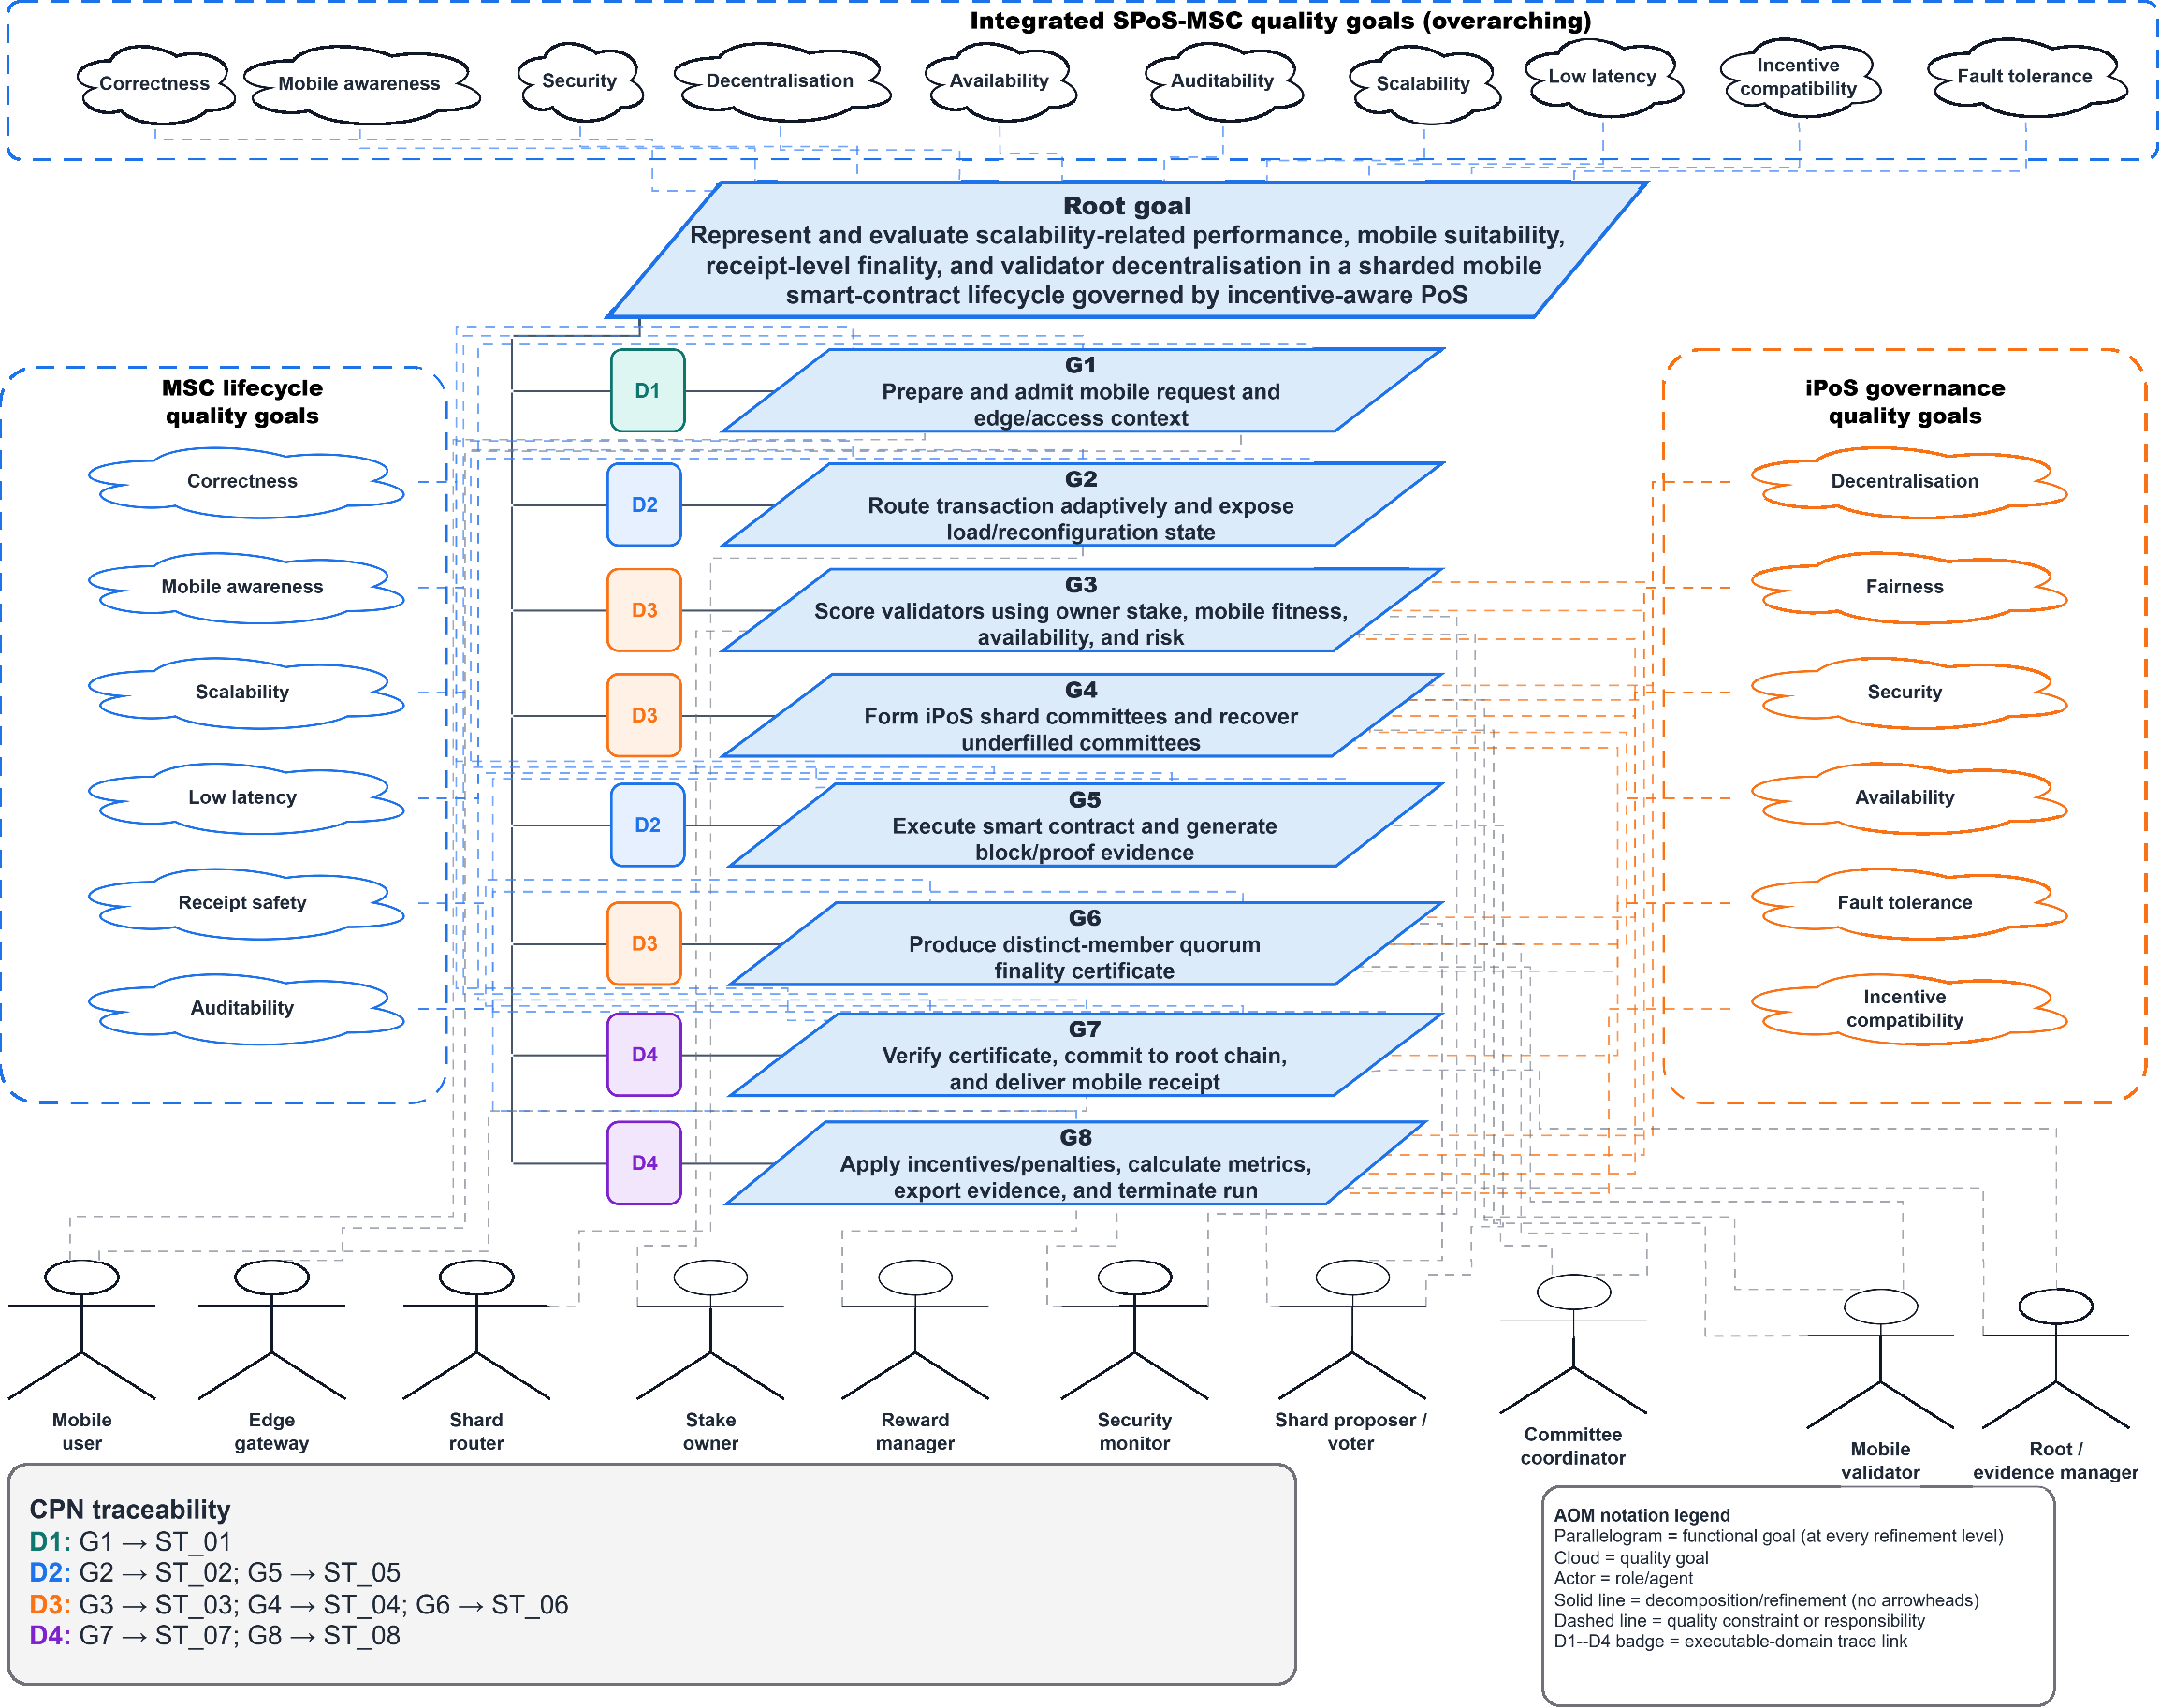
\includegraphics[width=\textwidth,height=0.72\textheight,keepaspectratio]
{figures/SPoS_MSC_Main_Goal_Model.pdf}
\caption{Integrated AOM goal model for SPoS-MSC. The root goal decomposes
into G1--G8, the D1--D4 badges identify executable domains, and the traceability
panel maps each functional goal to ST\_01--ST\_08. Parallelograms denote
functional goals, clouds denote quality goals, and dashed links denote quality
constraints or role responsibilities.}
\label{fig:spos_msc_goal}
\end{figure}

The integrated view in Fig.~\ref{fig:spos_msc_goal} is the primary AOM view of
this paper. Its root goal is to \emph{represent and evaluate
scalability-related performance, mobile suitability, receipt-level finality,
and validator decentralisation in a sharded mobile smart-contract lifecycle
governed by incentive-aware PoS}. This wording reflects the claim boundary. The study
evaluates a bounded four-shard configuration and scenario-level stress; it does
not claim an empirical scale-out advantage over external systems or unexecuted
internal baselines.

The root goal is decomposed into eight functional goals. In the executable hierarchy,
the goals are not merely numbered boxes: each one is assigned to a concrete
domain and substitution stage, as summarised in
Table~\ref{tab:goal_hierarchy}. The mapping also shows that scenario
initialisation is an experimental-control responsibility of ST\_01 rather than
a separate stakeholder goal. Its purpose is to create repeatable Q1--Q7 input
markings before the mobile-admission responsibility of G1 is exercised.

\begin{table*}[pos=t]
\centering
\caption{Alignment of the integrated AOM goals with the hierarchical CPN
execution domains and functional stages.}
\label{tab:goal_hierarchy}
\scriptsize
\setlength{\tabcolsep}{3.5pt}
\renewcommand{\arraystretch}{1.10}
\begin{tabularx}{\textwidth}{p{0.7cm}p{2.6cm}p{2.6cm}X p{3.2cm}}
\toprule
\textbf{Goal} & \textbf{Execution domain} & \textbf{CPN stage} &
\textbf{Functional responsibility} & \textbf{Principal quality constraints}\\
\midrule
G1 & D1 Mobile/access & ST\_01 &
Admit and prepare a mobile request after signature, wallet/deposit,
edge/access, resource, and connectivity checks; record explicit rejection
rather than losing an invalid request. &
Correctness, mobile awareness, availability, auditability.\\

G2 & D2 Shard routing/execution & ST\_02 &
Assign a prepared transaction using mapping, load, queue, latency,
cross-shard, and mobile-cost evidence; update the route state atomically when
reconfiguration is required. &
Scalability-related performance, low latency, correctness, auditability.\\

G3 & D3 iPoS governance/quorum & ST\_03 &
Score validators using owner-aggregated stake, capped nonlinear owner power,
mobile fitness, availability, risk, and fairness; separate benign exclusion
from quarantine and slashing. &
Fairness, decentralisation, security, mobile awareness.\\

G4 & D3 iPoS governance/quorum & ST\_04 &
Form seed-dependent shard committees and recover an underfilled committee from
the remaining eligible validators. &
Availability, fault tolerance, decentralisation, security.\\

G5 & D2 Shard routing/execution & ST\_05 &
Execute the model-level contract step and construct shard-block, state-hash,
and proof evidence, or record an explicit execution/proof failure. &
Correctness, security, low latency, auditability.\\

G6 & D3 iPoS governance/quorum & ST\_06 &
Create per-validator voting obligations and issue a finality certificate only
after the configured distinct-member quorum has been reached. &
Correctness, security, fault tolerance, availability.\\

G7 & D4 Root/receipt/evidence & ST\_07 &
Verify certificate--block--proof correspondence, commit accepted evidence to
the root chain, and deliver a verified mobile receipt or an explicit timeout. &
Receipt safety, correctness, mobile awareness, auditability.\\

G8 & D4 Root/receipt/evidence & ST\_08 &
Apply contribution rewards and penalties, update governance feedback,
calculate decentralisation/load metrics, export one run summary, and emit an
explicit completion token. &
Incentive compatibility, decentralisation, security, auditability.\\
\bottomrule
\end{tabularx}
\end{table*}

The domain grouping makes the cross-layer dependencies explicit. D1 produces
prepared transactions and validator/run context; D2 produces routed
transactions and block/proof evidence; D3 produces eligible committees, votes,
and quorum certificates; and D4 turns accepted certificates into root
commitments, receipts, incentive feedback, metrics, and completion evidence.
Accordingly, G6 is the principal consensus--lifecycle integration point, while
G7 and G8 carry the consequences of finality into mobile confirmation,
incentives, decentralisation measurement, and reproducible data collection.

The roles in the AOM view should be read in the same domain-oriented manner.
The mobile user and edge/access role contribute primarily to G1 and G7; the
shard router and shard executor contribute to G2 and G5; the stake owner,
validator, and committee coordinator contribute to G3, G4, and G6; and the
root/evidence, reward-management, and security-monitoring roles contribute to
G7 and G8. These responsibility links do not imply that each role is a separate
physical node in the CPN abstraction. They identify the logical
responsibilities whose interaction is represented by the executable model.

The quality goals remain correctness, mobile awareness, security,
decentralisation, availability, auditability, scalability-related performance,
low latency, incentive compatibility, and fault tolerance. Their placement in
the AOM view is not ornamental. Correctness and auditability constrain the
complete request-to-summary chain; mobile awareness constrains admission,
validator fitness, and receipt delivery; security and fault tolerance constrain
risk treatment, recovery, voting, and proof/certificate checks; and
incentive compatibility and decentralisation constrain owner-aware scoring,
reward feedback, and concentration measurement.

\subsection{Supporting MSC Lifecycle and iPoS Governance Views}
\label{subsec:supporting_goal_views}

The MSC lifecycle view and the iPoS governance view are retained as supporting
AOM artefacts in the supplementary material. They explain the origin of the
integrated goals without implying that the executable artefact consists of two
independent nets.

The lifecycle view follows the mobile request from creation to user-observable
completion. Its responsibilities are mobile admission and edge preparation,
adaptive shard routing, shard-local execution and proof construction,
committee-backed finality, root-chain commitment, and receipt delivery. These
responsibilities correspond primarily to G1, G2, G5, G6, and G7 and are
realised across D1, D2, D3, and D4. The lifecycle is therefore broader than
block inclusion: a transaction is not complete merely through routing or shard execution alone. It must either reach a verified receipt or produce an
explicit terminal outcome that explains why completion does not occur.

The iPoS governance view explains how validator state controls that lifecycle.
Its responsibilities include owner-level stake aggregation, capped nonlinear
power, mobile-fitness and risk assessment, eligibility filtering, seed-dependent
committee formation, recovery of underfilled committees, distinct-member
voting, proposer/voter/receipt rewards, penalties, and decentralisation
measurement. These responsibilities correspond primarily to G3, G4, G6, and
G8 and are realised in D3 and D4.

The two views meet through typed evidence rather than through an informal
architectural association. Block/proof evidence from G5 cannot become final
without the committee and voting state produced by G3--G6. A finality
certificate cannot become a mobile receipt without the verification and root
commitment of G7. Finally, the contributions and failures recorded during
G3--G7 become the reward, penalty, concentration, and completion evidence of
G8. This coupling distinguishes the hierarchical integration from a flat association of lifecycle and governance concerns.

\subsection{AOM-Derived Requirements and Executable Realisation}
\label{subsec:reqs}

The integrated and supporting views are refined into the ten requirements in Table~\ref{tab:reqs}. The requirements are intentionally limited to obligations that have both an executable representation and an observable output. The table
uses the hierarchy-level stage names rather than repeating every transition; Section~\ref{sec:cpn} gives the exact transitions, guards, inscriptions, and state types. This division avoids duplicating the formal model while preserving a direct requirements-to-implementation link. 

\begin{table*}[pos=t]
\centering
\caption{AOM-derived SPoS-MSC requirements, hierarchical CPN realisation, and
native evaluation evidence.}
\label{tab:reqs}
\scriptsize
\setlength{\tabcolsep}{3.2pt}
\renewcommand{\arraystretch}{1.10}
\begin{tabularx}{\textwidth}{p{0.65cm}p{2.5cm}p{3.5cm}p{4.4cm}X}
\toprule
\textbf{ID} & \textbf{Requirement} & \textbf{AOM obligation} &
\textbf{Hierarchical CPN realisation} & \textbf{Observable evidence}\\
\midrule
R1 & Mobile transaction preparation &
A submitted mobile request must be admitted only after symbolic signature,
wallet/deposit, edge/access, resource, and connectivity checks; otherwise it
must reach an explicit rejection outcome. &
D1/ST\_01; request archive, timed prepared-transaction state, preparation and
rejection paths. &
Submitted and prepared transactions, explicit terminal failures, and R1
evidence.\\

R2 & Shard routing and load awareness &
A prepared transaction must be assigned using current mapping and operating
conditions, while cross-shard and hotspot pressure remain observable. &
D2/ST\_02; route state, routed-transaction state, atomic reconfiguration, and
reconfiguration archive. &
Routed and cross-shard transactions, logical routing effects, shard-load
standard deviation, and reconfiguration events.\\

R3 & Proof-backed lifecycle finality &
Finality must be downstream of successful contract execution, block/proof
evidence, committee voting, and certificate/evidence verification. &
D2/ST\_05, D3/ST\_06, and D4/ST\_07; block/proof, certificate, and root archives
with explicit failure alternatives. &
Shard blocks, finality certificates, root commitments, finality success, and
finality latency.\\

R4 & Mobile receipt generation &
A mobile receipt must be generated only after accepted root commitment; poor
connectivity must result in an explicit delivery timeout rather than hidden
loss. &
D4/ST\_07; root work/archive, receipt-delivery work, verified receipt archive,
and timeout outcome. &
Receipts, receipt success, receipt latency, and terminal receipt-delivery
failures.\\

R5 & Owner-aware validator scoring &
Validator influence must reflect aggregated owner stake and capped nonlinear
owner power rather than raw per-validator stake alone. &
D3/ST\_03; owner aggregation and scoring functions, validator registry, and
score archive. &
Eligible-validator count, owner reward share, reward Gini, and reward HHI.\\

R6 & Mobile-fitness and risk-aware eligibility &
Committee participation must depend on mobile fitness, availability, and risk,
while benign weakness is distinguished from slashable behaviour. &
D3/ST\_03; eligibility guards, weak/offline exclusion, quarantine, penalty, and
security-evidence paths. &
Eligible-validator count, quarantine events, slashing events, and downstream
recovery demand.\\

R7 & Distinct-member committee-controlled finality &
Shard finality must depend on a seed-dependent committee, recovery when
underfilled, and a configured quorum of distinct affirmative voters. &
D3/ST\_04 and ST\_06; committee and recovery archives, per-validator vote tasks,
vote state, and certificate archive. &
Active committees, committee recoveries, vote/finality evidence, and finality
success.\\

R8 & Reward, slashing, and feedback &
Validators must receive contribution-linked rewards and behaviour-linked
penalties, with their balances updated for subsequent governance feedback. &
D4/ST\_08; reward and penalty tasks, reward/penalty archives, and balance-state
updates. &
Reward events, quarantine/slashing events, and concentration measures derived
from the updated reward balances.\\

R9 & Decentralisation monitoring &
The model must expose inequality, concentration, ownership, and
control-threshold evidence from the realised reward distribution. &
D4/ST\_08; CPN~ML functions for Gini, HHI, the 51\% Nakamoto coefficient,
largest-owner share, and load variation. &
Reward Gini, reward HHI, Nakamoto coefficient, largest-owner reward share, and
shard-load standard deviation.\\

R10 & Integrated evidence, experimental provenance, and termination & Lifecycle, consensus, security, performance, and parameter-configuration evidence must be recorded together, followed by explicit run completion. & D2/ST\_02 and D4/ST\_08; Run summary, sensitivity-data place, CSV line, reconfiguration evidence, stop code, experiment/factor/level identifiers, and serialised resolved configuration. & Lifecycle counts, throughput, latency, concentration, load dispersion, parameter vector, and invariant status. \\
\bottomrule
\end{tabularx}
\end{table*}

The table also clarifies several points that remain ambiguous in the earlier
requirements text. R3 now spans block/proof construction, quorum finality, and
root eligibility rather than treating a finality-certificate place as sufficient
evidence. R7 explicitly requires distinct-member quorum and committee recovery.
R10 includes explicit termination and data export, reflecting the native
replication procedure in which every run produces one summary only after the model consumes all pending
reward, penalty, reconfiguration, and transaction work. The sensitivity factors are executable evaluation controls rather than additional functional requirements. They vary selected parameters of R2, R4--R7, R9, and R10 while preserving the retained R1--R10 requirements and their traceability relations.

\subsection{Requirement-to-Evidence Coverage and Scope}
\label{subsec:traceability}

Let
\(
\mathcal{R}_{\mathrm{req}}=\{R1,\ldots,R10\}
\).
For every retained requirement, the model must provide at least one executable
realisation and one observable evidence item:
\begin{equation}
\forall r_i\in\mathcal{R}_{\mathrm{req}},\qquad
\tau(r_i)\neq\emptyset\ \wedge\ \mu(r_i)\neq\emptyset.
\end{equation}
Requirement coverage is therefore
\begin{equation}
TC=
\frac{
\left|\left\{r_i\in\mathcal{R}_{\mathrm{req}}\mid
\tau(r_i)\neq\emptyset\wedge\mu(r_i)\neq\emptyset\right\}\right|
}{|\mathcal{R}_{\mathrm{req}}|}.
\end{equation}
For the executable hierarchy, $TC=1$: all ten retained requirements are linked to
at least one CPN domain/stage and to at least one native run-level observation.
This value should be interpreted as \emph{traceability completeness}, not as a
claim that every quality goal is maximised in every scenario. For example, R4
is fully represented and observable even though poor connectivity can reduce
receipt delivery; R6 is traceable even when filtering risky validators narrows
the active set; and R10 is represented even when a transaction ends in an
explicit failure rather than a receipt.

The traceability chain used throughout the paper is therefore
\begin{equation}
\text{AOM goal}
\rightarrow
\text{requirement}
\rightarrow
\text{domain/stage and typed CPN state}
\rightarrow
\text{native run-level evidence}.
\end{equation}
Section~\ref{sec:cpn} defines the executable semantics of that chain, while
Sections~\ref{sec:methodology} and~\ref{sec:results} explain how the resulting
outputs are collected and interpreted. The abstraction boundary remains
explicit: production cryptography, peer-to-peer gossip, deployment-specific
wallet security, unbounded churn, and public-network scale-out are outside the
current requirements set. The model instead evaluates a bounded, reproducible
cross-layer lifecycle in which mobile admission, sharded execution, iPoS
governance, quorum finality, root commitment, receipt delivery, incentives,
and evidence completion are connected in one executable hierarchy.

% Keep Section 3 floats from drifting into Section 4.
\FloatBarrier


\section{Integrated SPoS-MSC Protocol and CPN Formalisation}
\label{sec:cpn}
\label{sec:framework}

Section~\ref{sec:aom} derives the SPoS-MSC requirements. This section addresses
RQ2 by translating them into one executable hierarchical Coloured Petri Net
(CPN). The public v4 model contains 13 pages, 171 places, 40 transitions,
380 arcs, 13 hierarchy instances, and 58 colour sets. It is not a
workspace containing disconnected MSC and PoS nets: one root instance invokes
a domain controller, which invokes four execution domains and eight functional
stages traced to G1--G8 and R1--R10. The presentation is organised around the
model hierarchy, typed CPN semantics, mobile-to-shard execution, iPoS
governance and quorum finality, and the root-to-evidence completion path.

\subsection{System Boundary and Hierarchical CPN Organisation}
\label{subsec:system_boundary}

Figure~\ref{fig:architecture} shows the system boundary. Mobile users submit
signed smart-contract requests through an edge/access layer. The shard domain
manages load-aware routing, contract execution, block construction, and proof
evidence. The iPoS governance domain performs owner-aware scoring,
mobile- and risk-aware filtering, VRF-style committee selection, recovery,
voting, and quorum finality. The root/evidence domain verifies certificates,
commits accepted evidence, delivers receipts, updates rewards and penalties,
calculates decentralisation metrics, and finalises each run.

\begin{figure}[pos=t]
\centering
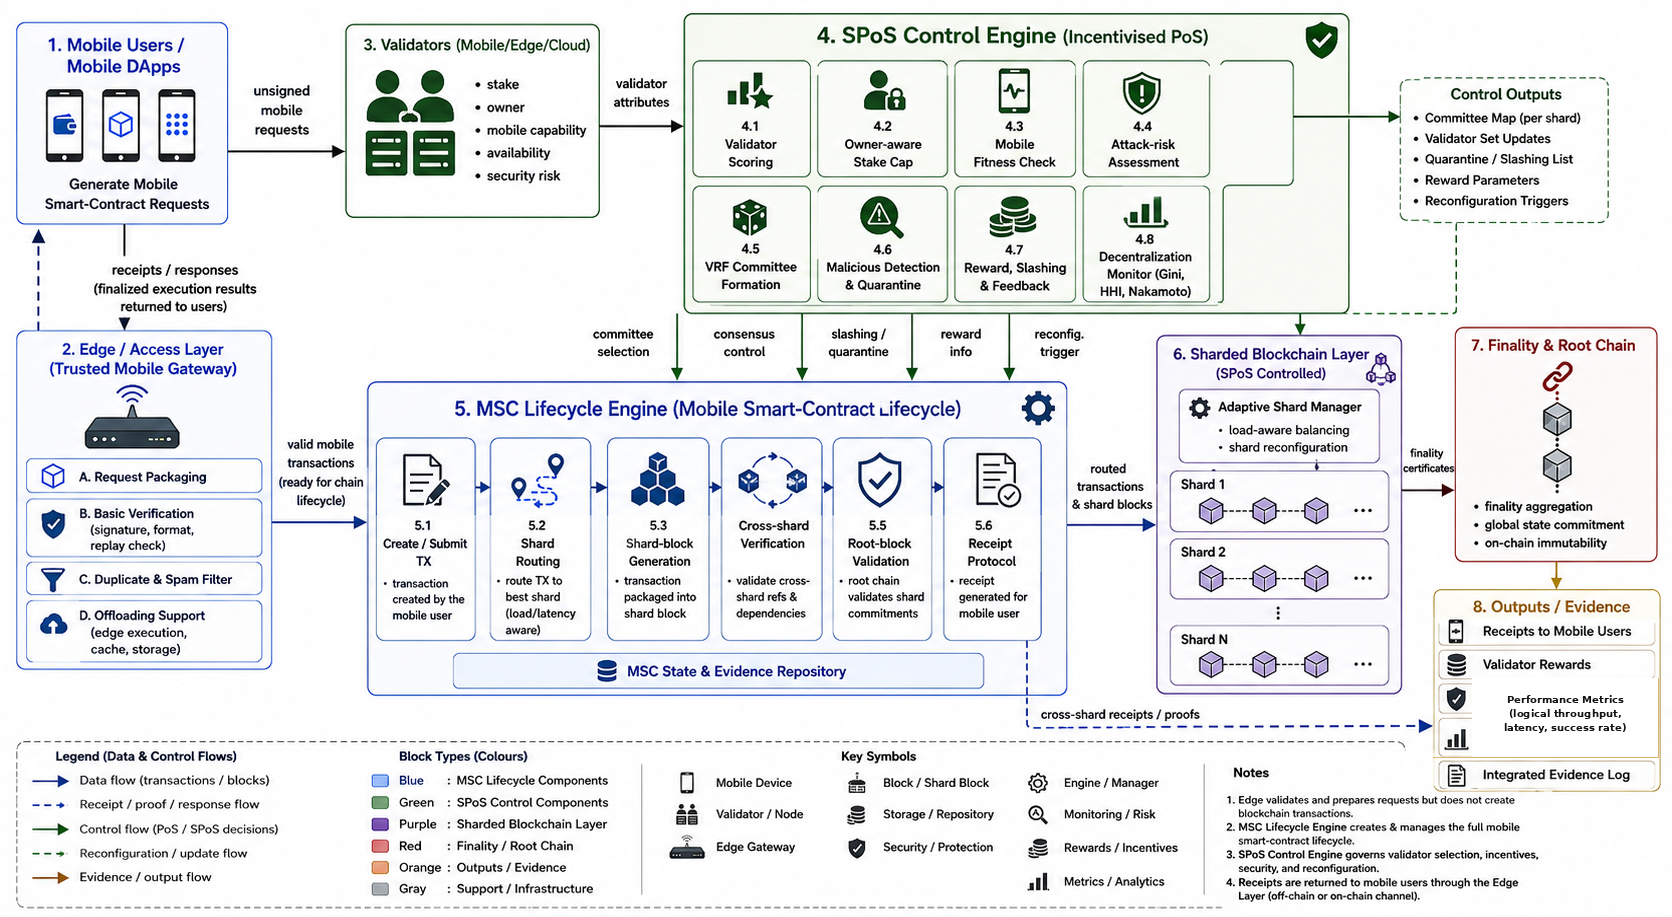
\includegraphics[width=\linewidth,height=0.60\textheight,keepaspectratio]
{figures/SPoS_MSC_Architecture.png}
\caption{SPoS-MSC system architecture and interaction among the mobile/access,
shard-execution, iPoS-governance, and root/evidence domains. Performance output
refers to logical completion rate, latency, and success rather than public-network TPS.}
\label{fig:architecture}
\end{figure}

The executable hierarchy is shown in Fig.~\ref{fig:cpn_hierarchy}. The root
page invokes the complete-lifecycle substitution transition, which instantiates
the domain controller. The controller then invokes four domain pages. D1
contains scenario generation and mobile request preparation; D2 contains
adaptive routing, reconfiguration, and shard execution; D3 contains owner-aware
scoring, committee recovery, and quorum finality; and D4 contains root
commitment, receipt delivery, incentives, metrics, and explicit termination.
Typed socket--port assignments carry prepared transactions, validator state,
block evidence, certificates, receipts, reward/penalty tasks, and run summaries
across the hierarchy. The exact CPN page and transition identifiers appear in
the hierarchy figure and supplementary executable artefact.

\begin{figure}[pos=htbp]
\centering
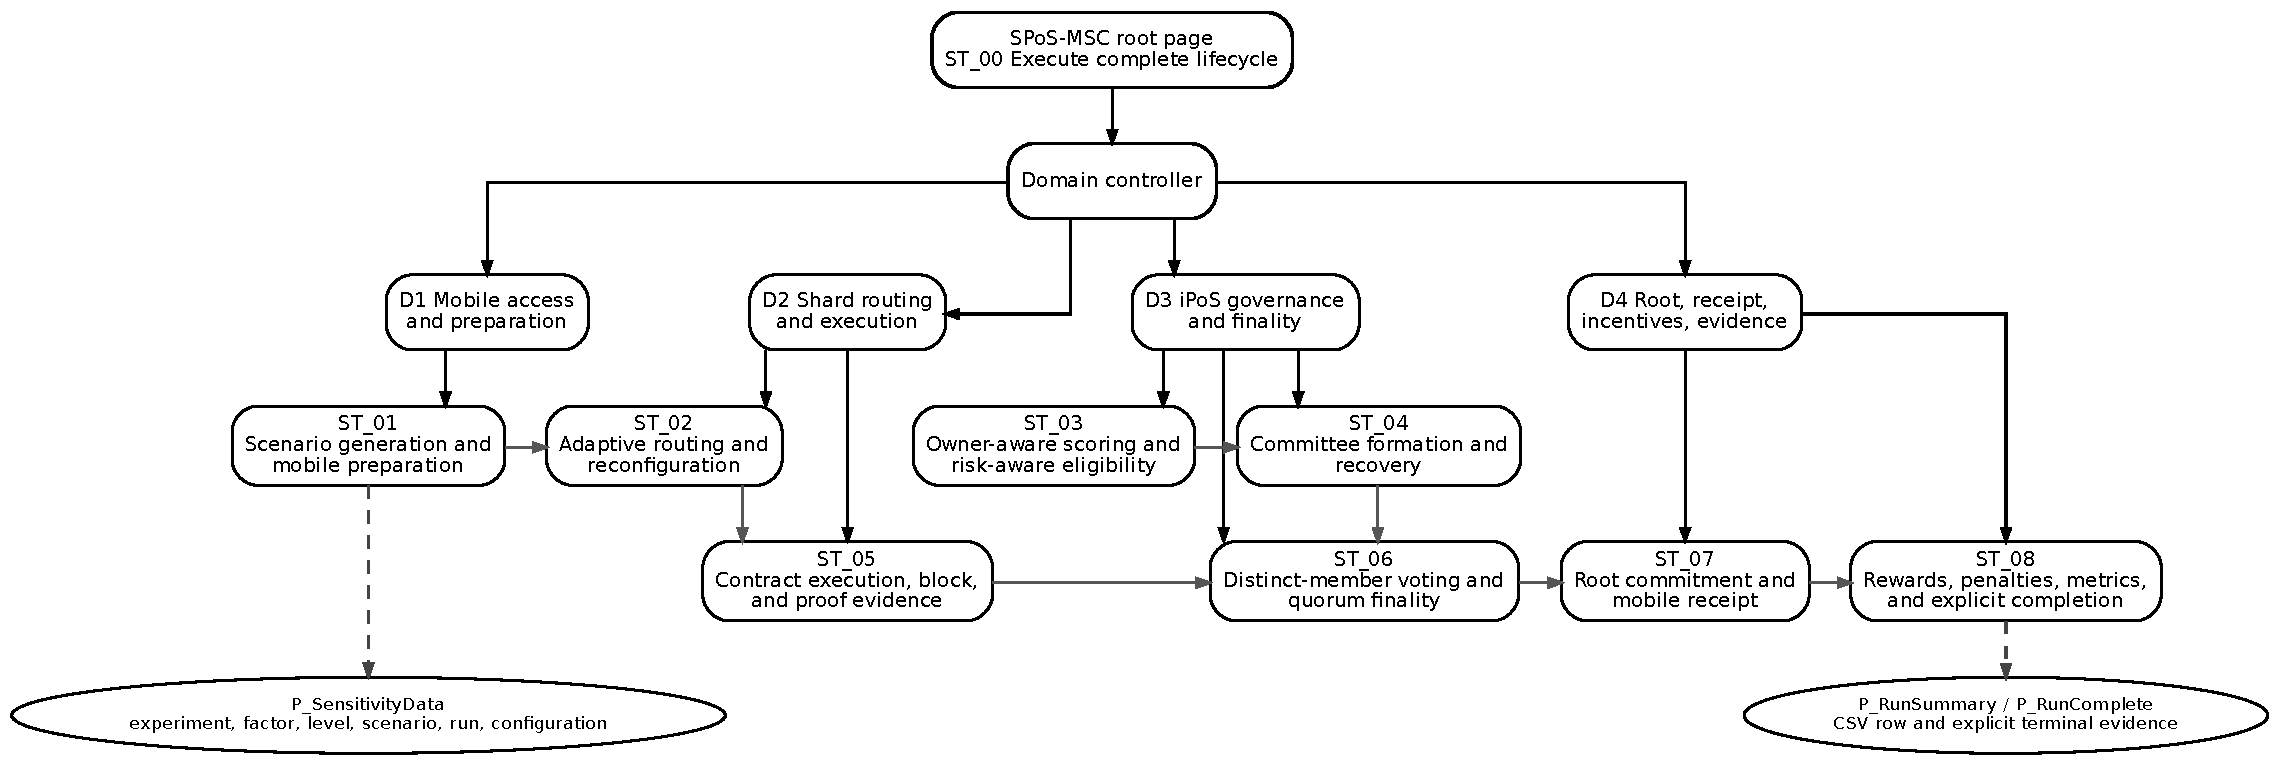
\includegraphics[width=0.98\textwidth]
{figures/SPoS_MSC_CPN_Hierarchy_v4.pdf}
\caption{Executable v4 hierarchy of the MSC lifecycle with incentive-aware PoS governance. The dashed observation paths expose the resolved sensitivity configuration and final run evidence without controlling lifecycle enabledness. Detailed CPN Tools pages and port--socket mappings appear in the supplementary artefacts.}
\label{fig:cpn_hierarchy}
\end{figure}

\subsection{Formal CPN Definition, Typed State, and Stage Semantics}
\label{subsec:cpn_definition}

The integrated model is represented as
\begin{equation}
CPN_{\mathrm{SPoS-MSC}}=(\Sigma,P,T,A,N,C,G,E,I,H,M),
\label{eq:cpn_tuple}
\end{equation}
where \(\Sigma\) is the set of colour sets, \(P\) the places, \(T\) the
transitions, \(A\) the arcs, \(N\) the arc-endpoint mapping, \(C\) the
place-colour assignment, \(G\) the transition guards, \(E\) the arc
inscriptions, \(I\) the initial marking, \(H\) the substitution-page mapping,
and \(M\) the archive and output places. A transition \(t\) is enabled in
marking \(m\) under binding \(b\) when the required input multisets are
available and its guard evaluates to true:
\begin{equation}
Enabled_m(t,b)\Leftrightarrow
\bigl(\forall p\in{}^{\bullet}t:\,m(p)\geq E(p,t)\langle b\rangle\bigr)
\wedge G(t)\langle b\rangle=\mathrm{true}.
\label{eq:cpn_enabled}
\end{equation}
Firing the enabled transition consumes the bound input multiset and produces the
bound output multiset:
\begin{equation}
m'=m-E^{-}(t,b)+E^{+}(t,b).
\label{eq:cpn_firing}
\end{equation}

The principal colour sets represent run configurations, mobile requests, timed
transactions, validators, owner-aware scores, committees, routed transactions,
block/proof evidence, vote tasks and vote states, finality certificates, root
commitments, receipts, reward and penalty tasks, security events, integrated
evidence, run summaries, and sensitivity-provenance tokens. Every transaction-linked token carries
\texttt{runId}, \texttt{scenarioId}, and \texttt{txId}; block, certificate,
root, and receipt tokens additionally retain matching shard, block, proof, or
commitment identifiers. These identifiers prevent evidence belonging to
unrelated transactions or replications from being combined. The transitions
\texttt{T\_InstantiateReplicationConfiguration} and
\texttt{T\_GenerateQ1\_Q7Scenario} create the scenario-dependent transaction,
validator, load, route, committee, timing, and seed state used by each native replication. Table~\ref{tab:transition_semantics} maps the eight requirements-facing stages to representative transitions in the executed model.

\begin{table*}[pos=t]
\centering
\caption{Requirements-facing stages and representative transitions in the
executed hierarchical CPN model.}
\label{tab:transition_semantics}
\scriptsize
\setlength{\tabcolsep}{3.2pt}
\renewcommand{\arraystretch}{1.10}
\begin{tabularx}{\textwidth}{p{2.5cm}p{5.6cm}X}
\toprule
\textbf{Stage} & \textbf{Representative executable transition(s)} &
\textbf{Role in the lifecycle} \\
\midrule
Scenario and mobile preparation &
\path{T_InstantiateReplicationConfiguration},
\path{T_GenerateQ1_Q7Scenario},
\path{T_PrepareValidMobileRequest} &
Creates a run-dependent Q1--Q7 configuration and admits or explicitly rejects
mobile requests after signature, wallet/deposit, edge, battery, CPU, and
connectivity checks.\\
Adaptive routing and reconfiguration &
\path{T_RouteByMappingLoadLatency},
\path{T_ApplyAtomicReconfiguration} &
Selects a shard from mapping, load, queue, latency, cross-shard, and mobile cost;
reconfiguration updates and returns the route state atomically.\\
Owner-aware scoring and risk &
\path{T_ScoreEligibleValidator},
\path{T_ExcludeWeakOrOfflineValidator},
\path{T_QuarantineAndSlashRiskyValidator} &
Aggregates stake by owner, applies nonlinear capped owner power, evaluates mobile
fitness and risk, and separates benign exclusion from quarantine/slashing.\\
Committee formation and recovery &
\path{T_FormVRFCommitteesAndRecover} &
Forms seed-dependent committees and records bounded recovery when a shard is
underfilled.\\
Smart-contract execution and proof &
\path{T_ExecuteContractBuildBlockAndProof},
\path{T_RecordExecutionFailure} &
Executes the model-level contract step and produces shard-block, state-hash, and
proof evidence or an explicit terminal failure.\\
Voting and quorum finality &
\path{T_VerifyEvidenceAndOpenVoting},
\path{T_CastHonestVote},
\path{T_ProduceQuorumFinalityCertificate},
\path{T_RecordNoQuorumFailure} &
Creates per-validator vote tasks and issues a certificate only after all expected
responses and the configured distinct-member quorum.\\
Root commitment and mobile receipt &
\path{T_VerifyCertificateAndScheduleRootCommit},
\path{T_CommitRootAndScheduleMobileReceipt},
\path{T_DeliverAndVerifyMobileReceipt},
\path{T_RecordReceiptTimeout} &
Verifies certificate/block/proof correspondence, commits accepted evidence, and
then delivers a verified receipt or records a timeout.\\
Incentives, metrics, and termination &
\path{T_ApplyContributionRewardAndFeedback},
\path{T_ApplyPenaltySlashingAndFeedback},
\path{T_FinalizeRunAndExposeMetrics} &
Applies proposer, voter, and receipt rewards, penalties, and stake feedback;
calculates concentration/load metrics; exports one run summary; and emits
\texttt{P\_RunComplete}.\\
\bottomrule
\end{tabularx}
\end{table*}

\subsection{Executable Parameterisation for Sensitivity Analysis}
\label{subsec:parameterisation}

To distinguish controlled parameter variation from the composite Q1--Q7 stress
scenarios, the v3 self-logging executable extends into the public v4 model
\texttt{\detokenize{SPoS_MSC_Hierarchical_Executable_v4_Sensitivity.cpn}}
(SHA-256:
\texttt{\detokenize{66eaa955bfd9269138437649cf6875d2d377c561a8b541944680be5eba114a10}}).
The public v4 executable contains 13 pages, 171 places, 40
transitions, 380 arcs, and 13 hierarchy instances. Relative to v3, the sensitivity layer adds observation and provenance structures
without introducing an additional lifecycle transition.

The colour set
\begin{equation}
\begin{split}
\texttt{IP\_SENSITIVITY}=\{&
\texttt{experimentId},\texttt{factorId},\texttt{levelId},\\
&\texttt{scenarioId},\texttt{runId},\texttt{config}\}
\end{split}
\end{equation}
records the experimental cell and a serialised copy of the resolved input
vector. Three hierarchy-connected places named
\texttt{P\_SensitivityData} propagate the token from the scenario-generation
page through D1 to the top page. These places have empty initial markings and
are output-only observations; they do not supply an enabling token to the
lifecycle. The same experiment, factor, level, scenario, run ID, and complete
configuration string are written into every native CSV row at run
finalisation.

The executable sensitivity controls are transaction count, forced cross-shard
demand, request-disconnection percentage, receipt-delivery-drop percentage,
owner-stake cap, minimum mobile-fitness threshold, committee/quorum, and
shard-load threshold. Their low, default, and high values are given in
Table~\ref{tab:sensitivity_design}. The sensitivity model passes a
two-run smoke test, a 72-run pilot, a 700-run default-configuration audit, and a
2,400-run OFAT experiment. All exported rows terminate with
\texttt{stop\_code=COMPLETE} and satisfy the lifecycle-ordering and terminal-
accounting invariants.

The v4 default-configuration audit reproduces the archived v3 core lifecycle totals exactly,
while four stochastic diagnostic totals differ: cross-shard transactions, reward
events, reconfiguration events, and integrated evidence records differ by
$-8$, $-13$, $-8$, and $-8$, respectively. Accordingly, the manuscript reports scenario and sensitivity results consistently from v4; the study does not claim bit-for-bit output equivalence with v3.


\subsection{Mobile Admission, Adaptive Routing, and Timed Shard Execution}
\label{subsec:routing_semantics}

A mobile request enters the executable lifecycle only when its symbolic
signature, wallet and deposit state, edge/access state, and device-resource
checks succeed. Valid requests are converted into timed prepared-transaction
tokens; invalid or unavailable requests are assigned an explicit terminal
outcome rather than remaining in an unexplained marking. The admission stage
therefore makes mobile feasibility part of the protocol state rather than an
external deployment assumption.

For candidate shard \(s\), the executable routing cost is
\begin{equation}
C(tx,s)=L_s+3Q_s+2D_s+C_{\mathrm{cross}}(tx,s)+C_{\mathrm{mobile}}(tx),
\label{eq:routing_cost}
\end{equation}
where \(L_s\), \(Q_s\), and \(D_s\) are the current load, queue, and latency
terms. The final terms represent cross-shard dependency and mobile/edge cost.
The selected shard minimises Eq.~\eqref{eq:routing_cost}. If a shard exceeds
the configured pressure threshold,
\texttt{T\_ApplyAtomicReconfiguration} consumes the current route state,
updates load, capacity, latency, mapping, and version information, and returns
the updated route state. This consume--update--return pattern prevents the
reconfiguration path from removing state needed by later transactions.

The routed transaction is then processed by
\texttt{T\_ExecuteContractBuildBlockAndProof}, which produces model-level
contract-execution status, shard-block identity, state-hash evidence, and proof
evidence. Execution failure is represented by a separate terminal path. Timed
arc inscriptions cover edge preparation, routing, block/proof generation,
quorum finality, root commitment, and receipt delivery. Cross-shard work,
high-load execution, and weak connectivity add scenario-dependent logical
delay; these values are model-time measurements rather than public-network
latency.

\subsection{Owner-Aware iPoS Governance, Committee Recovery, and Quorum Finality}
\label{subsec:validator_committee}

For owner \(o\), the model first aggregates the stake of all validators under
that owner:
\begin{equation}
S_o=\sum_{v_i\in V_o} stake_i.
\label{eq:owner_stake}
\end{equation}
The executable owner-power term caps and compresses this aggregate and shares it
across the owner's validator identities:
\begin{equation}
OwnerPower(v_i)=
\left\lfloor
\frac{\sqrt{100\min(S_{o_i},C_o)}}{\max(1,|V_{o_i}|)}
\right\rfloor .
\label{eq:owner_power}
\end{equation}
The mobile and integrated scores are
\begin{align}
Mobile(v_i)&=\max\left(0,
\left\lfloor\frac{battery_i+cpu_i+bandwidth_i+availability_i}{4}\right\rfloor
-\left\lfloor\frac{latency_i}{2}\right\rfloor\right),
\label{eq:mobile_score}\\
Score(v_i)&=OwnerPower(v_i)+Mobile(v_i)-risk_i+Fairness(v_i).
\label{eq:integrated_score}
\end{align}
A validator is eligible only if it is neither malicious/slashable nor offline,
has stake at least \(\theta_S\), satisfies \(Mobile(v_i)\geq\theta_M\), and
satisfies \(Score(v_i)\geq\theta_I\). The default configuration uses
\(C_o=3000\), \(\theta_S=10\), \(\theta_M=35\), and \(\theta_I=45\);
Table~\ref{tab:sensitivity_design} varies \(C_o\) and \(\theta_M\) in the local
OFAT experiment. Malicious or high-risk validators are quarantined and
penalised; benign weak or
offline validators follow a non-slashing exclusion path. Consequently, a
quarantined validator cannot enter the active committee set.

For each shard, a deterministic VRF-style ranking uses the base seed, run ID,
shard ID, validator ID, and score. If the initially selected set is underfilled,
recovery adds the best remaining eligible validators and records a recovery
event. Q1--Q5 and Q7 use committee size three and quorum two; Q6 uses committee
size four and quorum three. After shard-block and proof evidence are verified,
the model creates one vote task for each committee member. A finality
certificate is generated only after all expected responses have been recorded
and the number of distinct affirmative voters reaches the configured quorum:
\begin{equation}
Final(tx,s)\Rightarrow
\sum_{v_i\in C_{s,e}}\mathbf{1}[vote_i(tx)=\mathrm{YES}]\geq q_s.
\label{eq:quorum_finality}
\end{equation}
Thus, finality is controlled by the selected committee rather than by a single
validator token. Offline, invalid, and no-quorum outcomes remain observable
through separate penalty, security, and terminal-evidence paths.

\subsection{Root Commitment, Receipt Safety, Incentive Feedback, and Evidence Completion}
\label{subsec:finality_commitment}
\label{subsec:rewards_evidence}

The post-finality evidence path is structurally explicit. Using compact
transition labels for the executable transitions listed in
Table~\ref{tab:transition_semantics}, the path is
\begin{align}
P_{\mathrm{CertWork}}
&\xrightarrow{T_{\mathrm{verify}}}P_{\mathrm{RootWork}}
\xrightarrow{T_{\mathrm{commit}}}P_{\mathrm{ReceiptWork}}\nonumber\\
&\xrightarrow{T_{\mathrm{deliver}}}P_{\mathrm{ReceiptArchive}}.
\label{eq:receipt_path}
\end{align}
Certificate, block, proof, shard, run, and transaction identifiers must match
before root commitment is scheduled. Consequently,
\begin{equation}
Receipt(tx)\Rightarrow
\exists c,r:\ FinalityCertificate(c,tx)\wedge RootCommitment(r,c).
\label{eq:receipt_after_root}
\end{equation}
The poor-connectivity scenario may produce a receipt timeout after a valid root
commitment, thereby separating consensus finality from successful delivery to
the mobile participant.

The incentive path assigns five units to the proposer, two units to each
affirmative voter, and two additional units to the proposer when a receipt is
delivered. Offline or invalid voting and risk-based quarantine create separate
penalty tasks and update next-epoch balances. At finalisation, CPN ML calculates
reward Gini and HHI on a 0--100 scale, the Nakamoto coefficient at a 51\%
reward-share threshold, largest-owner reward share, and shard-load standard
deviation. Percentage-valued metrics are stored in the raw CSV in basis points.

A run finalises only after all expected transactions and validators reach
terminal or evaluated states, all reward, penalty, and reconfiguration tasks
have been consumed, committees have been built, and the run has not previously
been finalised. The emitted summary checks
\begin{equation}
N_{\mathrm{receipt}}\leq N_{\mathrm{root}}\leq N_{\mathrm{cert}}
\leq N_{\mathrm{block}}\leq N_{\mathrm{routed}}
\leq N_{\mathrm{prepared}}\leq N_{\mathrm{submitted}},
\label{eq:lifecycle_ordering}
\end{equation}
and terminal accounting additionally requires
\begin{equation}
N_{\mathrm{receipt}}+N_{\mathrm{terminal\ failure}}
=N_{\mathrm{submitted}}.
\label{eq:terminal_accounting}
\end{equation}
The principal archive and output places form three evidence groups:
(i) lifecycle archives for requests, preparation/routing, blocks, certificates,
root commitments, and receipts; (ii) governance and adaptation archives for
scores, committees, recovery, votes, rewards, penalties, and reconfiguration;
and (iii) provenance and completion places comprising
\path{P_SensitivityData}, \path{P_Evidence}, \path{P_RunSummary},
\path{P_RunSummaryCSVLine}, and \path{P_RunComplete}. The exact place names
and their hierarchy mappings appear in the supplementary executable artefact.
These properties are structural and run-observed safety arguments for the
bounded scenarios; they are not claims of exhaustive state-space verification
or production cryptographic correctness.

\FloatBarrier

\section{Evaluation Methodology}
\label{sec:methodology}

Section~\ref{sec:aom} derives the functional, quality, governance, and evidence
requirements of SPoS-MSC, while Section~\ref{sec:framework} realises those
requirements as the hierarchical CPN organised into four execution domains
(D1--D4) and eight functional stages (ST\_01--ST\_08). This section defines how
that executable model is evaluated to answer RQ3. In particular, the evaluation
examines whether complete lifecycle runs produce internally consistent evidence
about mobile request processing, shard execution, committee-controlled finality,
root commitment, receipt delivery, robustness, incentive feedback, and validator
decentralisation under the bounded Q1--Q7 scenarios.

The unit of analysis is one complete lifecycle replication rather than an
individual transaction, validator, or transition firing. A replication begins
with scenario-specific mobile requests, validators, ownership/stake values, and
shard state, and ends only when all expected transaction and validator work has
reached a terminal state and the model exposes an explicit run-completion token.
The primary evidence layer is native execution of the CPN model in CPN Tools. A
separate reference runtime emulator provides a secondary engineering sanity
check on the high-level lifecycle logic. The two layers are intentionally not
combined into a single performance claim because they use different execution
environments, workload scales, and time bases. Section~\ref{sec:results}
therefore reports the native CPN evidence first and treats the emulator results
as a separate cross-layer trend check.

\subsection{Evaluation Design, Evidence Layers, and Provenance}
\label{subsec:evaluation_design}

The final native evaluation uses CPN Tools 4.0.1 and the self-logging,
sensitivity-enabled executable
\begin{center}
\small
\texttt{\detokenize{SPoS_MSC_Hierarchical_Executable_v4_Sensitivity.cpn}}
\end{center}
The executable and primary native matrices are fixed by the following SHA-256
identifiers:
\begin{center}
\scriptsize
\renewcommand{\arraystretch}{1.08}
\begin{tabular}{@{}ll@{}}
\textbf{Artefact} & \textbf{SHA-256} \\
v4 executable CPN & \texttt{66eaa955bfd9269138437649cf6875d2d377c561a8b541944680be5eba114a10} \\
Two-run smoke CSV & \texttt{a0c0ccd7f2874f514c7b3be8f9559f23bce2e98e9f706dfca9aeae18e1f23326} \\
72-run pilot CSV & \texttt{3fd4f528822ec51992aa0567b54fe53e22f19eb1e0ce8b46bdabc80de966fe39} \\
700-run v4 default-configuration audit CSV & \texttt{b53668cd159f8dbf617c58e14694951f321152a6bddd5b0c7e1c40ef618e9481} \\
2,400-run OFAT CSV & \texttt{7ceae15f43505aaed676bd3aae9b8ba71244a0302ca896df743e35b8859a3bf7} \\
\end{tabular}
\end{center}
The hierarchy-connected \texttt{P\_SensitivityData} path exposes the
resolved configuration, while each CSV row records the experiment, factor,
level, complete parameter string, scenario, run ID, and all lifecycle, load,
resilience, and decentralisation outputs. The smoke and pilot matrices are
execution gates; the 700-run and 2,400-run matrices provide the reported
scenario and sensitivity evidence, respectively.

The archived v3 model and its 700-row matrix serve as predecessor artefacts in a provenance audit. The v4 default-configuration audit reproduces all core lifecycle totals of the archived v3 matrix---submitted, prepared, routed, block, finality, root, receipt, and terminal-failure counts---but four stochastic diagnostic totals differ. Relative to the archived v3 report, v4 records eight fewer cross-shard transactions, thirteen fewer reward events, eight fewer reconfigurations, and eight fewer integrated evidence records. The manuscript therefore uses the v4 700-run matrix consistently as the native scenario reference; it does not combine v3 scenario tables with v4 sensitivity results or claim exact output equivalence.

The model-level base seed is 626. For each scenario, the execution procedure sets the scenario identifier, resets the run counter, and evaluates
\texttt{CPN'Replications.}\allowbreak\texttt{nreplications~100}. Run IDs
therefore range from 1 to 100 within each of Q1--Q7, producing 700 separately
executed run summaries. The base seed and run ID enter the scenario generator
and deterministic VRF-style ranking functions, thereby varying requests,
validator attributes, and committee choices while preserving repeatability.

Native data collection is part of the executable termination semantics rather
than a separate manual transcription step. The low-priority transition
\texttt{\detokenize{T_FinalizeRunAndExposeMetrics}} is enabled only when its
completion guard holds. On firing, it produces one \texttt{IP\_RUNSUMMARY}
token in \texttt{P\_RunSummary}, writes one CSV row through the CPN ML
write-to-file hook exposed at \texttt{P\_RunSummaryCSVLine}, and places one
explicit completion token in \texttt{P\_RunComplete}. Each row records the
scenario and run identifiers, base seed, logical model time, stop code,
lifecycle counters, latency accumulators, reward-concentration measures,
owner-level concentration, and shard-load dispersion. The final reproducibility
archive should retain the exact executed model, the Q1--Q7 command script, the
unaltered 700-row CSV, replication reports and simulation-output directories,
CPN Tools version, checksum manifest, analysis code, and the tables and figures
derived from the raw matrix. Retaining the replication reports is important
because the CSV establishes internal consistency but cannot, by itself,
establish native CPN Tools provenance.

\subsection{Native Execution Protocol and Scenario Design}
\label{subsec:scenarios}

Each replication follows the same hierarchy formalised in
Section~\ref{sec:framework}. ST\_01 instantiates the replication configuration,
generates the Q1--Q7 request and validator inputs, and performs mobile request
admission in D1. D2 then applies adaptive shard routing and atomic
reconfiguration in ST\_02 and executes the smart contract with block/proof
evidence in ST\_05. D3 evaluates owner-aware validator suitability in ST\_03,
forms or recovers the shard committees in ST\_04, and applies distinct-member
quorum voting in ST\_06. Finally, D4 verifies the finality certificate, creates
the root commitment and mobile receipt in ST\_07, and applies reward, penalty,
decentralisation, and explicit-termination logic in ST\_08. The experiment thus
observes the complete requirements-to-output path rather than testing the
stages as disconnected components.

All scenarios use four shards and ten input validators. The scenario generator
then varies the offered workload, transaction dependencies, mobile
connectivity, owner/stake distribution, validator risk and availability,
committee/quorum requirement, and shard-reconfiguration pressure. The exact
bounded configuration is given in Table~\ref{tab:scenario_parameters}.

\begin{table*}[pos=t]
\centering
\caption{Native Q1--Q7 CPN scenario matrix. Each scenario includes 100 replications.}
\label{tab:scenario_parameters}
\scriptsize
\setlength{\tabcolsep}{3.2pt}
\renewcommand{\arraystretch}{1.10}
\begin{tabularx}{\textwidth}{llrrrrrrX}
\toprule
\textbf{Sc.} & \textbf{Name} & \textbf{Tx/run} & \textbf{Val.} &
\textbf{Shards} & \textbf{Comm./quorum} & \textbf{Load th.} &
\textbf{Max. time} & \textbf{Primary stress mechanism} \\
\midrule
Q1 & Normal & 24 & 10 & 4 & 3/2 & 75 & 180 & Nominal end-to-end lifecycle \\
Q2 & High load & 40 & 10 & 4 & 3/2 & 75 & 180 & Increased offered-load pressure \\
Q3 & Cross-shard & 28 & 10 & 4 & 3/2 & 75 & 180 & Cross-contract and cross-shard dependencies \\
Q4 & Poor connectivity & 24 & 10 & 4 & 3/2 & 75 & 240 & Admission degradation and receipt timeout \\
Q5 & Stake skew & 24 & 10 & 4 & 3/2 & 75 & 180 & Shared ownership with concentrated high stake \\
Q6 & Risky/offline & 24 & 10 & 4 & 4/3 & 75 & 180 & Risk exclusion, quarantine, and committee recovery \\
Q7 & Hot shard & 32 & 10 & 4 & 3/2 & 55 & 180 & Hotspot pressure and adaptive reconfiguration \\
\bottomrule
\end{tabularx}
\end{table*}

Q1 exercises the nominal path across all four domains and is used as the
internal reference condition. Q2 increases the number of requests without
changing the shard count; Q3 deliberately raises cross-contract dependencies;
and Q7 concentrates mappings on a hot shard while lowering the load threshold.
These three scenarios primarily stress routing, execution, latency, and
reconfiguration in D2. Q4 targets the mobile boundary by degrading request
connectivity and receipt delivery. Q5 stresses owner-aware scoring and reward
concentration, whereas Q6 injects malicious and offline validators and raises
the committee/quorum requirement from 3/2 to 4/3 to exercise exclusion,
recovery, and quorum formation in D3. Because the shard count remains fixed at
four, the experiment is a bounded scalability-related stress study and not an
empirical shard scale-out experiment.

\subsection{Local One-Factor-at-a-Time Sensitivity Design}
\label{subsec:sensitivity_design}

The Q1--Q7 experiment evaluates seven composite stress conditions, whereas a
parameter-sensitivity experiment must vary one executable input while holding
the remaining logged configuration fixed. A local one-factor-at-a-time (OFAT)
experiment therefore evaluates eight controls. Each factor is
evaluated at low, default, and high levels in the scenario that directly
activates the corresponding mechanism. The design contains $8\times3=24$
configurations and 100 native CPN replications per configuration, for 2,400
runs. The shard count and input-validator count remain fixed at four and ten,
respectively.

\begin{table*}[pos=t]
\centering
\caption{Local OFAT sensitivity design. Each factor--level cell contains 100
native CPN replications.}
\label{tab:sensitivity_design}
\scriptsize
\setlength{\tabcolsep}{3.0pt}
\renewcommand{\arraystretch}{1.10}
\begin{tabularx}{\textwidth}{p{2.8cm}p{0.9cm}p{1.35cm}p{1.35cm}p{1.35cm}X}
\toprule
\textbf{Factor} & \textbf{Anchor} & \textbf{Low} & \textbf{Default} &
\textbf{High} & \textbf{Pre-specified primary response}\\
\midrule
Transactions per run & Q1 & 16 & 24 & 40 & Logical throughput\\
Forced cross-shard demand (\%) & Q3 & 20 & 60 & 80 & Receipt latency\\
Request disconnection (\%) & Q4 & 10 & 20 & 30 & Finality success\\
Receipt delivery drop (\%) & Q4 & 10 & 29 & 40 & Receipt success\\
Owner-stake cap & Q5 & 1500 & 3000 & 6000 & Largest-owner reward share\\
Mobile-fitness threshold & Q6 & 25 & 35 & 65 & Eligible validators\\
Committee/quorum & Q6 & 3/2 & 4/3 & 5/4 & Committee recovery\\
Load threshold & Q7 & 45 & 55 & 75 & Reconfiguration events\\
\bottomrule
\end{tabularx}
\end{table*}

The model-level base seed remains 626 and run IDs are reset to 1--100 within
each factor--level cell. However, separately executed cells with identical
logged configurations do not produce row-wise identical stochastic
diagnostics for the same run ID. The run ID is therefore retained for
provenance and coverage validation, but the cells are not treated as matched
pairs or as a common-random-number design. The three levels of each factor are
analysed as independent repeated-run groups.

For each factor, an omnibus Kruskal--Wallis test evaluates differences among
the low, default, and high levels. The associated local effect size is
\begin{equation}
\epsilon^2=\frac{H-k+1}{N-k},
\label{eq:sensitivity_epsilon}
\end{equation}
where $H$ is the Kruskal--Wallis statistic, $k=3$, and $N=300$. Low and high
levels are then compared separately with the factor-specific default using
two-sided Mann--Whitney $U$ tests. Holm correction is applied across the
sixteen pre-specified non-default contrasts, and Cliff's delta reports
stochastic effect size. To preserve the original measurement scale, each
contrast is also reported as a difference in group means with a two-sided
Welch 95\% confidence interval. These procedures do not require row-wise
pairing and are suitable for bounded percentages, integer counts, and
continuous run-level outputs.

The smoke, pilot, default-audit, and OFAT matrices contain 2, 72, 700, and
2,400 rows, respectively. Every row has base seed 626 and
\texttt{stop\_code=COMPLETE}; the validation detects no lifecycle-ordering, terminal-accounting, or
duplicate configuration/run-key violation. The 72-run pilot is
used only as a parameter-logging and termination gate. Inferential sensitivity
results are calculated from the 2,400-run matrix. Because one factor is varied
at a time over three selected levels, the experiment establishes local
sensitivity within the reported intervals; it is not a Sobol, Morris, or other
global sensitivity analysis and it does not estimate higher-order
interactions.

\subsection{Measures and Run-Level Data Collection}
\label{subsec:metrics}

The recorded measures follow the same lifecycle, scalability, governance, and
evidence dimensions introduced in Sections~\ref{sec:aom} and
\ref{sec:framework}. Lifecycle performance is represented by finality success,
receipt success, logical throughput, finality latency, and receipt latency.
Scalability-related stress is represented by the cross-shard ratio, shard-load
standard deviation, and reconfiguration events. Governance and resilience are
represented by eligible validators, active committees, committee recoveries,
quarantine events, and slashing events. Incentive and decentralisation evidence
is represented by reward events, reward Gini, reward HHI, the Nakamoto
coefficient, and the largest-owner reward share. The evidence counter and stop
code provide an additional audit trail for requirements-to-output traceability
and explicit completion.

For run $r$, the principal rate and timing measures are defined as
\begin{align}
F_r & = 100\,\frac{N_{\mathrm{cert},r}}{N_{\mathrm{submitted},r}},
&
R_r & = 100\,\frac{N_{\mathrm{receipt},r}}{N_{\mathrm{submitted},r}},
\label{eq:success_rates}\\
X_r & = 100\,\frac{N_{\mathrm{cross},r}}{N_{\mathrm{submitted},r}},
&
\Theta_r^{\mathrm{CPN}} & =
\frac{N_{\mathrm{receipt},r}}{T_{\mathrm{model},r}},
\label{eq:stress_throughput}\\
L_{F,r} & =
\frac{A_{F,r}}{n_{F,r}},
&
L_{R,r} & =
\frac{A_{R,r}}{n_{R,r}},
\label{eq:latency_measures}
\end{align}
where $F_r$ and $R_r$ are the finality and receipt success percentages,
$X_r$ is the percentage of submitted transactions classified as cross-shard,
$\Theta_r^{\mathrm{CPN}}$ is receipt completion per unit of logical CPN time,
and $A_F$, $A_R$, $n_F$, and $n_R$ are the corresponding latency sums and
observation counts. Latency means use their corresponding observation counts. To avoid division
by zero, the analysis script records a missing value when an observation count is
non-positive; that run is excluded only from the affected latency summary and is
not interpreted as having zero processing delay. Logical CPN time is obtained from the
model clock and is not wall-clock time; consequently,
$\Theta_r^{\mathrm{CPN}}$ is a model-level completion rate and not blockchain
transactions per second.

Reward Gini, reward HHI, and largest-owner reward share are reported on a
0--100 scale. The raw CSV stores these values as integers scaled by 100, so they
are divided by 100 during analysis. The Nakamoto coefficient is the minimum
number of validators whose descending reward shares reach the configured 51\%
threshold. Shard-load standard deviation is likewise rescaled from its integer
CSV representation before reporting. Scenario-level tables use the 100 run-level
observations. When Section~\ref{sec:results} reports a transaction-weighted
aggregate success rate across scenarios, it is calculated from the sums of the
corresponding counts rather than by averaging scenario percentages.

\subsection{Statistical Analysis and Integrity Validation}
\label{subsec:data_collection}

For every scenario and run-level metric, the analysis reports the mean,
standard deviation, median, interquartile range, minimum, and maximum. The
reported two-sided 95\% confidence interval for a scenario mean is
\begin{equation}
\bar{x}\;\pm\;t_{0.975,99}\frac{s}{\sqrt{100}},
\label{eq:t_confidence_interval}
\end{equation}
where $\bar{x}$ is the mean of the 100 replications, $s$ is the sample standard
deviation, and $t_{0.975,99}$ is the Student-$t$ critical value with 99 degrees
of freedom. The complete descriptive matrix is supplied as supplementary data.
Transactions, votes, or receipts generated within the same replication are not
treated as independent statistical observations. The study is descriptive and
scenario-based; it does not use the confidence intervals to claim causal
superiority over an unexecuted protocol variant.

Integrity validation precedes the statistical calculations. At the
model level, \texttt{T\_FinalizeRunAnd}\hspace{0pt}\texttt{ExposeMetrics} can fire only when all
expected transactions are terminal, all validators have been evaluated, all
pending reward, penalty, and reconfiguration tasks have been consumed,
committees have been built, and the run has not already been finalised. The
native stop-code invariant then requires
\begin{equation}
N_{\mathrm{receipt}}
\leq N_{\mathrm{root}}
\leq N_{\mathrm{cert}}
\leq N_{\mathrm{block}}
\leq N_{\mathrm{routed}}
\leq N_{\mathrm{submitted}}.
\label{eq:native_lifecycle_invariant}
\end{equation}
Post-processing additionally applies checks that are not encoded in the native
stop-code invariant. These require
$N_{\mathrm{prepared}}\leq N_{\mathrm{submitted}}$,
$N_{\mathrm{cross}}\leq N_{\mathrm{routed}}$, and
$N_{\mathrm{receipt}}+N_{\mathrm{terminal\ failure}}=
N_{\mathrm{submitted}}$, together with non-negative counters, valid scenario and
run identifiers, and the expected replication cardinality. This distinction is
important: Equation~\eqref{eq:native_lifecycle_invariant} is evaluated inside
the CPN at finalisation, whereas the additional conditions are applied to each
exported row before aggregation.

The v4 default-configuration audit CSV contains exactly 700 rows, with 100 rows for each
scenario, run IDs 1--100 within each scenario, base seed 626, and
\texttt{stop\_code=COMPLETE} in every row. The validation detects no lifecycle-ordering, terminal-accounting, schema, or
range violation. These checks
support the internal consistency of the analysed matrix; they remain
run-observed validation checks and are not presented as exhaustive state-space
verification or production cryptographic correctness.

The sensitivity exports are validated independently from the original scenario
matrix. For the OFAT study, the expected cardinality is 2,400 rows arranged as
24 factor--level groups of 100 run IDs. The validator checks the logged
factor and level, complete parameter vector, unique key, run-ID coverage,
\texttt{COMPLETE} status, non-negative counters, lifecycle ordering, and terminal
accounting before any descriptive or sensitivity statistic is calculated. No
factorial interaction matrix is reported in this manuscript; interaction
analysis remains future work.

\subsection{Comparison Strategy and Reference Runtime Boundary}
\label{subsec:baselines}
\label{subsec:experimental_environment}

The native experiment compares the complete SPoS-MSC model across Q1--Q7 and
uses Q1 only as the nominal internal reference. Q2--Q7 are stress conditions,
not independently implemented protocol baselines. The local OFAT sensitivity
experiment isolates parameter changes within the full model; it is not an
executable protocol ablation or competing-consensus baseline. In particular, the native
experiment does not execute single-chain, stake-only, Round-Robin,
static-routing, or no-reconfiguration variants. The analysis therefore does not
attribute observed differences causally to SPoS-MSC relative to those
alternatives. Systems discussed in the related-work comparison are used only to
contextualise capability coverage and metric families because their hardware,
shard counts, validator populations, workloads, network assumptions, and
finality definitions are different.

The secondary artefact is a Python/FastAPI reference runtime emulator that executes
in memory on an x86\_64 Linux host with 56 CPU cores and 4~GB memory. It follows
the same high-level sequence of request preparation, routing, validator
assessment, committee formation, finality, root commitment, receipt handling,
and reward/penalty feedback. It does not implement distributed shard nodes,
peer-to-peer propagation, persistent blockchain state, production signatures
or VRF proofs, networked committee messages, or production root-chain
consensus. Its receipts/s value is therefore an in-memory lifecycle-event
processing rate rather than public-network blockchain throughput.

The CPN and emulator use analogous Q1--Q7 labels but different workload scales,
execution mechanisms, and time bases. Cross-layer comparisons are consequently
limited to descriptive trend consistency, such as whether the same stress
families affect completion, latency, cross-shard activity, or concentration;
they are not numerical equivalence tests. The defensible claims from this
evaluation are therefore limited to complete-lifecycle reachability and
ordering, bounded stress behaviour, governance and incentive evidence,
decentralisation measurement, and traceability from the requirements and CPN
semantics to the exported outputs. The study does not claim public-network
throughput superiority, production deployment equivalence, or empirical
scale-out beyond the evaluated four-shard configuration.


\section{Results and Discussion}
\label{sec:results}

Section~\ref{sec:methodology} defines native CPN Tools execution as the
primary evidence layer and the reference runtime emulator as a secondary
engineering check. It also defines the complete replication as the unit of
analysis, Q1 as the nominal internal reference, and Q2--Q7 as bounded stress
conditions rather than independently implemented protocol baselines. The
results are therefore organised along the requirements-to-model-to-evidence
chain developed in Sections~\ref{sec:aom} and~\ref{sec:framework}. Native
execution completeness and requirement traceability are reported first,
followed by lifecycle performance, scalability-related stress and resilience,
incentive/decentralisation behaviour, the completed local sensitivity analysis,
and the cross-layer trend check. The
section then positions the evidence relative to related work, answers RQ3, and
states the validity boundaries under which the findings should be interpreted.

\subsection{Native Execution Completeness and Requirement Traceability}
\label{subsec:lifecycle_trace}
\label{subsec:req_satisfaction_results}

A representative Q1 trace traverses the complete hierarchy from scenario
instantiation and mobile request preparation in D1, through adaptive routing and
contract execution in D2, owner-aware scoring and committee-controlled finality
in D3, to root commitment, receipt delivery, incentive feedback, metric export,
and explicit run completion in D4. More importantly, every replication reaches the same terminal protocol: the native output matrix contains 700 run
summaries, all with \texttt{stop\_code=COMPLETE}, and the validation detects no
lifecycle-ordering or terminal-accounting violation. Run completion here means that all
expected work reached a modelled terminal state; it does not mean that every
submitted transaction succeeded.

\begin{table*}[pos=t]
\centering
\caption{Aggregate native CPN evidence across 700 v4 SPoS-MSC replications.}
\label{tab:cpn_aggregate_native}
\footnotesize
\setlength{\tabcolsep}{5pt}
\renewcommand{\arraystretch}{1.08}
\begin{tabularx}{\textwidth}{Xr@{\hspace{1.0cm}}Xr}
\toprule
\textbf{Metric} & \textbf{Value} & \textbf{Metric} & \textbf{Value}\\
\midrule
Scenario replications & 700 & Submitted transactions & 19,600\\
Prepared/routed transactions & 18,941 & Shard blocks & 18,767\\
Finality certificates & 18,767 & Root commitments & 18,767\\
Mobile receipts & 18,187 & Terminal failures & 1,413\\
Weighted finality success & 95.75\% & Weighted receipt success & 92.79\%\\
Aggregate logical throughput & 0.461 & Cross-shard ratio & 25.44\%\\
Weighted finality latency & 22.59 & Weighted receipt latency & 38.00\\
Reward events & 94,899 & Committee recoveries & 115\\
Quarantine/slashing events & 200/200 & Reconfiguration events & 1,393\\
Integrated evidence records & 316,366 & Invariant-valid completed runs & 700\\
\bottomrule
\end{tabularx}
\end{table*}

Table~\ref{tab:cpn_aggregate_native} exposes where the 1,413 terminal failures
occur. The gap of 659 between submitted and prepared transactions is
concentrated in the poor-connectivity condition, where requests can fail the
mobile admission path. A further 174 prepared and routed transactions do not reach block/finality evidence; these failures occur under the high-load
condition. Finally, 580 transactions reached a finality certificate and root
commitment but did not produce a mobile receipt, corresponding to the explicit
delivery-timeout path in Q4. Hence,
$659+174+580=1{,}413$, and every unsuccessful request is represented by a
modelled terminal outcome rather than by an unexplained dead marking. The equal
counts for blocks, finality certificates, and root commitments also agree with
the ordering invariant defined in Section~\ref{subsec:data_collection}.

Table~\ref{tab:reqsat} closes the traceability loop from the AOM requirements in
Section~\ref{sec:aom} to the native outputs. The table reports evidence coverage,
not production-level certification: a requirement is considered covered when
its CPN realisation is exercised and at least one corresponding run-level output
is exposed within the evaluated abstraction.

\begin{table*}[pos=t]
\centering
\caption{Run-observed native CPN evidence for the AOM-derived requirements
R1--R10.}
\label{tab:reqsat}
\scriptsize
\setlength{\tabcolsep}{3.2pt}
\renewcommand{\arraystretch}{1.10}
\begin{tabularx}{\textwidth}{p{0.65cm}p{2.75cm}X p{2.35cm}}
\toprule
\textbf{Req.} & \textbf{Requirement} & \textbf{Observed evidence} &
\textbf{Most informative scenario(s)}\\
\midrule
R1 & Mobile transaction preparation & Submitted, prepared, rejected, and
terminal request outcomes are exported for each replication, including the
admission-failure path. & Q1, Q4\\
R2 & Shard routing and load awareness & Routed transactions, cross-shard
activity, shard-load dispersion, and atomic reconfiguration events are exposed. &
Q2, Q3, Q7\\
R3 & Proof-backed lifecycle finality & Contract execution produces block/proof
evidence before quorum certification and root commitment; the corresponding
counts and latencies are exported. & Q1--Q7\\
R4 & Mobile receipt generation & A receipt is recorded only after root
commitment, while mobile delivery timeout is retained as a distinct terminal
outcome. & Q1, Q4\\
R5 & Owner-aware validator scoring & Owner stake/power, eligible-validator
counts, reward concentration, and largest-owner reward share are calculated; Q5
groups three high-stake validators under one owner. & Q5\\
R6 & Mobile-fitness and risk-aware eligibility & Weak or offline validators are
excluded from the active path, while risky validators are quarantined and
penalised. & Q6\\
R7 & Committee-controlled shard finality & Committee size, quorum,
distinct-member voting, underfilled-committee recovery, and no-quorum outcomes
are represented and observable. & Q6\\
R8 & Reward, slashing, and feedback & Proposer, voter, and receipt rewards, as
well as penalty/slashing tasks, update validator balances and produce auditable
events. & Q5--Q7\\
R9 & Decentralisation monitoring & Reward Gini, reward HHI, the 51\% Nakamoto
coefficient, and largest-owner reward share are generated from each completed
run. & Q5--Q7\\
R10 & Integrated evidence, provenance, and termination & Lifecycle, governance, security, load, incentive, and resolved parameter evidence is exported with reconfiguration records, one run summary, one sensitivity-data token, and one explicit completion token after pending work is consumed. & Q1--Q7 and OFAT\\
\bottomrule
\end{tabularx}
\end{table*}

The observed matrix provides non-empty evaluation evidence for all ten retained
requirements. Together with the requirement-to-CPN mappings established in
Section~\ref{subsec:traceability}, this gives evaluation-side traceability
coverage of $TC=10/10=1$ within the modelled scope. This result should be read as
completeness of the requirements-to-output chain. It does not extend the claim
to concrete cryptographic verification, wide-area peer-to-peer behaviour, or
other deployment properties that lie outside the retained R1--R10 scope.

\subsection{Lifecycle Performance Across Q1--Q7}
\label{subsec:cpn_results}

Table~\ref{tab:cpn_performance_native} reports the run-level means and 95\%
confidence-interval half-widths defined in Section~\ref{subsec:metrics}. The
success percentages use submitted transactions as their denominator, while
logical throughput is the number of receipts per unit of CPN model time. The
figures visualise the same run-level distributions; none of these rates should
be interpreted as public-network transactions per second.

\begin{table*}[pos=t]
\centering
\caption{Native v4 CPN lifecycle performance over 100 replications per scenario. Values are means $\pm$ 95\% confidence-interval half-widths.}
\label{tab:cpn_performance_native}
\scriptsize
\setlength{\tabcolsep}{3.2pt}
\renewcommand{\arraystretch}{1.10}
\begin{tabular}{llccccc}
\toprule
\textbf{Sc.} & \textbf{Name} & \textbf{Finality (\%)} & \textbf{Receipt (\%)} & \textbf{Logical throughput} & \textbf{Finality latency} & \textbf{Receipt latency}\\
\midrule
Q1 & Normal & 100.00 $\pm$ 0.00 & 100.00 $\pm$ 0.00 & 0.4444 $\pm$ 0.0105 & 19.32 $\pm$ 0.16 & 33.52 $\pm$ 0.23\\
Q2 & High load & 95.65 $\pm$ 0.22 & 95.65 $\pm$ 0.22 & 0.6262 $\pm$ 0.0118 & 22.69 $\pm$ 0.14 & 37.21 $\pm$ 0.20\\
Q3 & Cross-shard & 100.00 $\pm$ 0.00 & 100.00 $\pm$ 0.00 & 0.4883 $\pm$ 0.0108 & 26.51 $\pm$ 0.05 & 43.95 $\pm$ 0.08\\
Q4 & Poor connectivity & 72.54 $\pm$ 0.56 & 48.38 $\pm$ 0.59 & 0.1908 $\pm$ 0.0046 & 26.30 $\pm$ 0.15 & 46.08 $\pm$ 0.30\\
Q5 & Stake skew & 100.00 $\pm$ 0.00 & 100.00 $\pm$ 0.00 & 0.4510 $\pm$ 0.0102 & 19.37 $\pm$ 0.14 & 33.59 $\pm$ 0.20\\
Q6 & Risky/offline & 100.00 $\pm$ 0.00 & 100.00 $\pm$ 0.00 & 0.4470 $\pm$ 0.0101 & 19.40 $\pm$ 0.16 & 33.63 $\pm$ 0.23\\
Q7 & Hot shard & 100.00 $\pm$ 0.00 & 100.00 $\pm$ 0.00 & 0.6397 $\pm$ 0.0004 & 24.27 $\pm$ 0.05 & 40.74 $\pm$ 0.07\\
\bottomrule
\end{tabular}
\end{table*}

\begin{figure}[pos=htbp]
\centering

\includegraphics[width=\linewidth]{figures/Fig4_CPN_Logical_Throughput_v4.pdf}
\caption{Native CPN logical throughput across Q1--Q7. Error bars show 95\%
confidence intervals over 100 replications.}
\label{fig:cpn_throughput_native}
\end{figure}

\begin{figure}[pos=htbp]
\centering
\begin{minipage}{0.49\textwidth}
\centering

\includegraphics[width=\linewidth]{figures/Fig5a_CPN_Finality_Receipt_Success_v4.pdf}
\end{minipage}\hfill
\begin{minipage}{0.49\textwidth}
\centering

\includegraphics[width=\linewidth]{figures/Fig5b_CPN_Finality_Receipt_Latency_v4.pdf}
\end{minipage}
\caption{Native CPN lifecycle outcomes: finality and receipt success (left),
and logical finality and receipt latency (right).}
\label{fig:cpn_success_latency_native}
\end{figure}

Q1 establishes the nominal request-to-receipt behaviour: every submitted
transaction reaches finality and receipt, with mean logical throughput 0.444,
mean finality latency 19.32, and mean receipt latency 33.52. Q5 and Q6 remain
close to this lifecycle profile even though their governance inputs differ.
This shows that stake skew and the evaluated risky/offline population did not,
within these bounded runs, prevent completion of the transactions that entered
the lifecycle. The governance consequences of those scenarios are considered
separately in Sections~\ref{subsec:scalability_results} and
\ref{subsec:decentralisation_results}.

Under Q2, increasing the offered workload from 24 to 40 transactions per run
raises the measured logical completion rate from 0.444 to 0.626, approximately
41\% above Q1. This higher rate is accompanied by lower success: 174 routed
transactions fail before finality, yielding finality and receipt success of
95.65\%. Finality and receipt latencies also rise to 22.69 and 37.21. The
scenario therefore demonstrates that a larger number of receipts can be
completed per unit of logical time while a small proportion of the offered
workload still fails; throughput and completion probability are not
interchangeable measures.

Q3 separates cross-shard coordination cost from transaction loss. All submitted
transactions reach finality and receipt even though cross-shard activity rises
to 63.29\%. Relative to Q1, mean finality latency increases from 19.32 to 26.51
and receipt latency from 33.52 to 43.95. In the evaluated four-shard setting,
the cross-shard scenario therefore manifests primarily as additional logical
delay rather than reduced completion.

Q4 is the principal liveness bottleneck. Only 72.54\% of submitted requests
reach finality and 48.38\% produce receipts, while logical throughput falls to
0.191. The 24.16 percentage-point gap between finality and receipt success is
important: some requests pass committee finality and root commitment but still
terminate at mobile delivery timeout. Thus, receipt success is a stricter
end-to-end measure than finality success for the mobile lifecycle. Q4 also has
the highest receipt latency, 46.08, among successful receipt observations.

Q7 records the highest logical throughput, 0.640, and 100\% completion, but its
latencies remain higher than the nominal case. As shown below, this result
coexists with substantial cross-shard activity, load dispersion, and
reconfiguration. It should therefore be interpreted as successful completion
under a bounded hot-shard workload, not as evidence that hotspot cost has been
eliminated or that the system scales out with additional shards.

\FloatBarrier

\subsection{Shard Pressure, Reconfiguration, and Validator Resilience}
\label{subsec:scalability_results}

The lifecycle results become more informative when read together with the
stress and resilience measures in Table~\ref{tab:cpn_scalability_security_native}.
Cross-shard ratio captures dependency pressure, load standard deviation captures
dispersion across the four shards, and reconfiguration records the activation of
the adaptive-routing path. Eligible-validator, recovery, quarantine, and
slashing counts expose how the governance layer responds to the Q6 validator
population.

\begin{table*}[pos=t]
\centering
\caption{Native v4 shard pressure, reconfiguration, and validator-resilience evidence. Values are means $\pm$ 95\% confidence-interval half-widths.}
\label{tab:cpn_scalability_security_native}
\scriptsize
\setlength{\tabcolsep}{3.0pt}
\begin{tabular}{llccccccc}
\toprule
\textbf{Sc.} & \textbf{Name} & \textbf{Cross-shard (\%)} & \textbf{Reconfig./run} & \textbf{Load SD} & \textbf{Eligible val.} & \textbf{Recovery/run} & \textbf{Quarantine/run} & \textbf{Slashing/run}\\
\midrule
Q1 & Normal & 11.62 $\pm$ 1.22 & 0.05 $\pm$ 0.04 & 2.68 $\pm$ 0.24 & 10 & 0.00 $\pm$ 0.00 & 0 & 0\\
Q2 & High load & 15.45 $\pm$ 1.05 & 5.48 $\pm$ 0.17 & 8.11 $\pm$ 0.54 & 10 & 0.00 $\pm$ 0.00 & 0 & 0\\
Q3 & Cross-shard & 63.29 $\pm$ 0.44 & 0.58 $\pm$ 0.11 & 5.90 $\pm$ 0.60 & 10 & 0.00 $\pm$ 0.00 & 0 & 0\\
Q4 & Poor connectivity & 7.92 $\pm$ 0.85 & 0.00 $\pm$ 0.00 & 2.95 $\pm$ 0.11 & 10 & 0.00 $\pm$ 0.00 & 0 & 0\\
Q5 & Stake skew & 11.92 $\pm$ 1.06 & 0.02 $\pm$ 0.03 & 2.46 $\pm$ 0.22 & 10 & 0.00 $\pm$ 0.00 & 0 & 0\\
Q6 & Risky/offline & 12.25 $\pm$ 1.22 & 0.04 $\pm$ 0.04 & 2.71 $\pm$ 0.23 & 6 & 1.15 $\pm$ 0.11 & 2 & 2\\
Q7 & Hot shard & 48.38 $\pm$ 0.42 & 7.76 $\pm$ 0.19 & 9.51 $\pm$ 0.34 & 10 & 0.00 $\pm$ 0.00 & 0 & 0\\
\bottomrule
\end{tabular}
\end{table*}

\begin{figure}[pos=htbp]
\centering
\begin{minipage}{0.49\textwidth}
\centering

\includegraphics[width=\linewidth]{figures/Fig6a_CPN_Cross_Shard_Ratio_v4.pdf}
\end{minipage}\hfill
\begin{minipage}{0.49\textwidth}
\centering

\includegraphics[width=\linewidth]{figures/Fig6b_CPN_Reconfiguration_Load_Imbalance_v4.pdf}
\end{minipage}
\caption{Native CPN scalability-related stress evidence: cross-shard activity
(left), and load dispersion and reconfiguration (right).}
\label{fig:cpn_scalability_native}
\end{figure}

Q2 and Q7 account for 1,324 of the 1,393 reconfiguration events, approximately
95\% of the aggregate total. Q2 combines a moderate cross-shard ratio of 15.45\%
with 5.48 reconfigurations per run and load SD 8.11, indicating that offered-load
pressure, rather than cross-shard dependency alone, activates the routing
response. Q7 produces the strongest combined load signal: cross-shard activity
is 48.38\%, load SD reaches 9.51, and reconfiguration rises to 7.76 events per
run. Its 100\% receipt success therefore coexists with persistent hotspot cost.
The model makes overload visible and records corrective action, but the current
experiment does not compare that action with a disabled-reconfiguration
counterfactual.

Q3 shows a different stress pattern. It has the highest cross-shard ratio,
63.29\%, but only 0.58 reconfigurations per run and lower load dispersion than
Q2 and Q7. Combined with the latency results in
Table~\ref{tab:cpn_performance_native}, this indicates that the designed
cross-shard condition chiefly exercises dependency-related delay, whereas the
high-load and hot-shard conditions more strongly exercise the load-threshold and
reconfiguration paths. Q4, by contrast, produces no reconfiguration because its
failures originate at mobile admission and receipt delivery rather than shard
overload.

Q6 directly exercises validator resilience. The eligible set falls from ten to
six, two validators per run are quarantined and slashed, and the model performs
1.15 committee recoveries per run on average under the larger 4/3
committee/quorum requirement. Nevertheless, all Q6 transactions reach finality
and receipt. This is run-observed evidence that the exclusion and recovery paths
can coexist with liveness in the evaluated population. It is not a general proof
that recovery will succeed for arbitrary offline fractions, adversarial
strategies, or committee sizes. In relation to the structural properties in
Sections~\ref{subsec:validator_committee} and~\ref{subsec:finality_commitment}, Q6 exercises quarantine exclusion
and committee-dependent finality, while Q2 and Q7 exercise overload
observability.

\FloatBarrier

\subsection{Incentive and Decentralisation Trade-offs}
\label{subsec:decentralisation_results}

Table~\ref{tab:cpn_decentralisation_native} reports four complementary views of
reward concentration. Gini and HHI describe the validator-level reward
distribution, the Nakamoto coefficient gives the minimum number of validators
whose cumulative rewards reach the configured 51\% threshold, and
largest-owner share aggregates rewards across validators controlled by the same
owner. Reading the measures together is necessary because a distribution can be
comparatively even across validator identities while remaining concentrated at
the owner level.

\begin{table*}[pos=t]
\centering
\caption{Native v4 reward and owner-concentration evidence. Values are means $\pm$ 95\% confidence-interval half-widths.}
\label{tab:cpn_decentralisation_native}
\scriptsize
\setlength{\tabcolsep}{4.0pt}
\begin{tabular}{llcccc}
\toprule
\textbf{Sc.} & \textbf{Name} & \textbf{Reward Gini} & \textbf{Reward HHI} & \textbf{Nakamoto (51\%)} & \textbf{Largest-owner reward share (\%)}\\
\midrule
Q1 & Normal & 50.29 $\pm$ 1.14 & 19.29 $\pm$ 0.54 & 2.57 $\pm$ 0.10 & 28.80 $\pm$ 1.23\\
Q2 & High load & 50.33 $\pm$ 1.15 & 19.32 $\pm$ 0.56 & 2.57 $\pm$ 0.10 & 29.07 $\pm$ 1.27\\
Q3 & Cross-shard & 50.13 $\pm$ 1.18 & 19.28 $\pm$ 0.56 & 2.56 $\pm$ 0.10 & 28.90 $\pm$ 1.31\\
Q4 & Poor connectivity & 50.00 $\pm$ 1.12 & 19.11 $\pm$ 0.53 & 2.59 $\pm$ 0.10 & 29.26 $\pm$ 1.15\\
Q5 & Stake skew & 46.95 $\pm$ 0.81 & 17.43 $\pm$ 0.28 & 2.93 $\pm$ 0.05 & 45.82 $\pm$ 2.19\\
Q6 & Risky/offline & 59.99 $\pm$ 0.64 & 23.22 $\pm$ 0.45 & 2.14 $\pm$ 0.07 & 35.60 $\pm$ 1.07\\
Q7 & Hot shard & 56.87 $\pm$ 1.03 & 23.96 $\pm$ 0.72 & 1.98 $\pm$ 0.04 & 40.59 $\pm$ 1.03\\
\bottomrule
\end{tabular}
\end{table*}

\begin{figure}[pos=htbp]
\centering

\includegraphics[width=\linewidth]{figures/Fig7_CPN_Reward_Gini_HHI_v4.pdf}
\caption{Reward Gini and HHI across Q1--Q7 with 95\% confidence intervals.}
\label{fig:cpn_concentration_native}
\end{figure}

Q1--Q4 form a relatively stable reference band: mean Gini is approximately
50.0--50.3, mean HHI approximately 19.1--19.3, the Nakamoto coefficient
approximately 2.6, and largest-owner share approximately 29\%. This stability
suggests that workload size, cross-shard dependency, and mobile-connectivity
stress do not by themselves substantially alter the reward distribution in the
current reward abstraction.

Q5 reveals why validator- and owner-level measures must not be conflated. Under
the shared-owner stake-skew configuration, Q5 has the lowest validator-level
Gini (46.95) and HHI (17.43) and the highest Nakamoto coefficient (2.93), yet its
largest-owner reward share rises to 45.82\%. The evaluated owner-aware scoring
therefore distributes rewards across validator identities without eliminating
the concentration created by common ownership. These data do not establish
causal improvement over stake-proportional selection because the experiment
does not execute a stake-only variant; instead, they show that the model exposes
remaining owner-level concentration rather than hiding it behind
validator-level metrics.

Q6 and Q7 exhibit the opposite trade-off. Q6 reduces the eligible population to
six and records mean Gini 59.99, HHI 23.22, and Nakamoto coefficient 2.14. Q7
records mean Gini 56.87, HHI 23.96, and a Nakamoto coefficient of 1.98. In Q6,
the concentration increase accompanies risk-based exclusion and committee
recovery; in Q7, it accompanies hotspot-concentrated work and frequent
reconfiguration. Thus, stronger filtering or uneven execution demand can
preserve lifecycle completion while narrowing the set of rewarded contributors.
The decentralisation result is consequently a multi-metric security/load--
participation trade-off, not uniform improvement across all scenarios.

\FloatBarrier

\subsection{Local Parameter Sensitivity and Robustness}
\label{subsec:sensitivity_results}

The Q1--Q7 matrix establishes behaviour under composite stress conditions. The
2,400-run OFAT matrix addresses the complementary question of how the principal
outputs respond when one executable parameter is varied while the remaining
logged configuration is held fixed. All 24 factor--level cells contain 100
completed runs and no lifecycle-ordering or terminal-accounting violation.
Table~\ref{tab:sensitivity_primary} reports each factor's pre-specified primary
response. Every omnibus Kruskal--Wallis test is significant at $p<0.001$.

\begin{table*}[pos=t]
\centering
\caption{Local OFAT sensitivity results for the pre-specified primary response of each factor. Each level includes 100 independent native CPN replications.}
\label{tab:sensitivity_primary}
\scriptsize
\setlength{\tabcolsep}{2.6pt}
\renewcommand{\arraystretch}{1.10}
\begin{tabularx}{\textwidth}{p{2.55cm}p{2.55cm}ccccl}
\toprule
\textbf{Factor} & \textbf{Primary response} & \textbf{Low} & \textbf{Default} & \textbf{High} & $\boldsymbol{\epsilon^2}$ & \textbf{High--default difference (95\% CI)}\\
\midrule
Transactions/run & Logical throughput & 0.334 & 0.445 & 0.681 & 0.898 & 0.235 [0.218, 0.252]\\
Cross-shard demand & Receipt latency & 37.36 & 43.98 & 47.29 & 0.889 & 3.309 [3.158, 3.459]\\
Request disconnection & Finality success (\%) & 81.75 & 72.54 & 63.29 & 0.836 & -9.250 [-10.36, -8.142]\\
Receipt delivery drop & Receipt success (\%) & 63.88 & 48.38 & 39.83 & 0.841 & -8.542 [-9.575, -7.508]\\
Owner-stake cap & Largest-owner reward share (\%) & 33.05 & 45.56 & 38.96 & 0.192 & -6.596 [-9.601, -3.592]\\
Mobile-fitness threshold & Eligible validators & 6.000 & 6.000 & 3.000 & 1.000 & -3.000 [-3.000, -3.000]\\
Committee/quorum & Committee recoveries/run & 0.480 & 1.150 & 2.250 & 0.630 & 1.100 [0.925, 1.275]\\
Load threshold & Reconfiguration events/run & 10.17 & 7.860 & 4.150 & 0.863 & -3.710 [-3.917, -3.503]\\
\bottomrule
\end{tabularx}
\begin{minipage}{0.98\textwidth}\footnotesize
All Kruskal--Wallis omnibus tests have $p<0.001$. Non-default versus default contrasts use Mann--Whitney $U$ tests with Holm adjustment and Cliff's delta; the displayed confidence interval is a Welch interval for the difference in means. The analysis is local to the tested levels and is not a global variance decomposition.
\end{minipage}
\end{table*}

\begin{figure}[pos=htbp]
\centering

\includegraphics[width=\linewidth]{figures/Fig8_Sensitivity_Primary_Effect_Size_v4.pdf}
\caption{Local OFAT sensitivity of the pre-specified primary responses. The
Kruskal--Wallis $\epsilon^2$ values compare the three tested levels of each
factor; they are local effect sizes, not global Sobol indices.}
\label{fig:sensitivity_effect_size}
\end{figure}

Workload, cross-shard demand, mobile connectivity, receipt delivery, and load
threshold produce strong monotonic responses in their associated metric. Raising
workload from 24 to 40 transactions increases mean logical throughput from
0.445 to 0.681, a difference of 0.235 [0.218, 0.252], but also raises receipt
latency from 33.80 to 35.23 and reconfiguration from 0.01 to 5.51 events per
run. This result is specific to the Q1 anchor: unlike composite Q2, the workload
sweep does not activate additional pre-finality failure rules, and all three
levels retain 100\% completion. Increasing forced cross-shard demand from 60\%
to 80\% raises the observed cross-shard ratio from 63.50\% to 80.86\% and
receipt latency by 3.31 [3.16, 3.46] logical-time units while preserving 100\%
finality and receipt completion. Thus, within the four-shard model, cross-shard
pressure is expressed primarily as delay rather than loss.

The two connectivity controls separate admission and delivery sensitivity.
Increasing request disconnection from 20\% to 30\% reduces finality success from
72.54\% to 63.29\% (difference $-9.25$ percentage points, 95\% CI
$[-10.36,-8.14]$) and increases terminal failures from 12.39 to 13.84 per run.
Increasing receipt drop from 29\% to 40\% leaves finality success unchanged at
72.54\% but reduces receipt success from 48.38\% to 39.83\% (difference
$-8.54$ percentage points, 95\% CI $[-9.58,-7.51]$). This confirms that mobile
receipt delivery is a distinct end-to-end liveness boundary rather than a proxy
for consensus finality.

The sharpest governance tipping point occurs at the mobile-fitness threshold.
Thresholds 25 and 35 both retain six eligible validators and 100\% completion,
showing that the lower interval is inactive for the generated Q6 population. At
65, eligibility falls to three validators, finality and receipt success fall to
75\%, committee recovery rises from 1.15 to 4.00 events per run, reward Gini
rises from 59.97 to 76.96, reward HHI from 23.23 to 40.57, the Nakamoto
coefficient falls from 2.16 to 1.34, and largest-owner reward share rises from
35.79\% to 52.44\%. The finding identifies a threshold-dependent
security--availability--decentralisation trade-off rather than supporting an
unqualified recommendation for stricter mobile eligibility.

\begin{figure}[pos=htbp]
\centering
\begin{minipage}{0.49\textwidth}
\centering

\includegraphics[width=\linewidth]{figures/Fig9a_Sensitivity_MobileThreshold_Success_v4.pdf}
\end{minipage}\hfill
\begin{minipage}{0.49\textwidth}
\centering

\includegraphics[width=\linewidth]{figures/Fig9b_Sensitivity_MobileThreshold_Concentration_v4.pdf}
\end{minipage}
\caption{Mobile-fitness-threshold sensitivity: lifecycle success and eligible validators (left), and validator/owner concentration measures (right). Error bars show 95\% confidence intervals over 100 independent replications per level.}
\label{fig:sensitivity_mobile_threshold}
\end{figure}

Committee/quorum and load threshold expose different control trade-offs.
Moving from 4/3 to 5/4 committees increases recovery by 1.10 [0.93, 1.27]
events per run and slightly reduces throughput, but it lowers Gini from 59.90
to 56.49, HHI from 23.15 to 21.14, and owner share from 35.53\% to 34.36\%,
while raising the Nakamoto coefficient from 2.15 to 2.28. For the hot-shard
scenario, increasing the load threshold from 55 to 75 reduces reconfiguration
from 7.86 to 4.15 events per run, but load dispersion increases from 9.31 to
14.02, throughput falls from 0.640 to 0.586, and receipt latency rises from
40.72 to 42.30. Conversely, the lower threshold of 45 triggers more frequent
reconfiguration (10.17) but lowers load dispersion (5.61). The adaptive policy
therefore trades intervention frequency against imbalance and delay.

Owner-cap sensitivity is statistically significant but non-monotonic. The
largest-owner share is 33.05\%, 45.56\%, and 38.96\% at caps 1500, 3000, and
6000, respectively. The default cap is therefore the most concentrated of the
three tested points, while lifecycle completion remains 100\% throughout. This
should not be simplified to a claim that increasing the cap always increases or
always decreases concentration; the result reflects interaction between the
cap, owner grouping, scoring, and committee/reward assignment. A denser cap
sweep or factorial analysis is required to characterise that response surface.

Overall, lifecycle ordering and terminal accounting are robust across all 2,400
runs. Completion is locally stable to workload, cross-shard demand, owner cap,
committee/quorum, and load threshold over the tested ranges, but it is sensitive
to mobile disconnection, receipt loss, and an overly strict mobile-fitness
threshold. These conclusions are local to the stated levels and do not replace
protocol ablations, shard scale-out, or global sensitivity analysis.


\FloatBarrier

\subsection{Reference Runtime Emulator and Cross-Layer Trend Check}
\label{subsec:implementation_results}

The reference runtime emulator runs separately from the native CPN
runs, as required by Section~\ref{subsec:experimental_environment}. Its results
are reported to assess whether the scenario family produces broadly consistent
engineering trends in an independently coded lifecycle. The receipts/s column
is an in-memory event-processing rate on the stated host and is not blockchain
throughput.

\begin{table*}[pos=t]
\centering
\caption{Reference runtime emulator over 100 executions per scenario. The event
rate is an in-memory lifecycle-processing rate, not public-network TPS.}
\label{tab:realtime}
\scriptsize
\setlength{\tabcolsep}{4.0pt}
\renewcommand{\arraystretch}{1.08}
\begin{tabular}{llrrrrrr}
\toprule
\textbf{Sc.} & \textbf{Name} & \textbf{ms/run} & \textbf{Receipts/s} &
\textbf{Receipt (\%)} & \textbf{Receipt lat.} & \textbf{Cross (\%)} & \textbf{Gini}\\
\midrule
Q1 & Normal & 8.65 & 26030.48 & 96.33 & 23.21 & 12.19 & 29.85\\
Q2 & High load & 13.19 & 33141.69 & 96.37 & 23.60 & 19.20 & 28.92\\
Q3 & Cross-shard & 9.73 & 27945.65 & 95.16 & 25.30 & 47.64 & 28.94\\
Q4 & Poor connectivity & 8.43 & 24365.21 & 80.98 & 26.89 & 15.20 & 29.67\\
Q5 & Stake skew & 9.83 & 31207.60 & 96.51 & 23.44 & 16.26 & 28.87\\
Q6 & Risky/offline & 9.38 & 29894.39 & 96.30 & 23.63 & 19.31 & 29.05\\
Q7 & Hot shard & 12.08 & 29906.57 & 92.36 & 23.83 & 23.00 & 30.10\\
\bottomrule
\end{tabular}
\end{table*}

At the scenario-mean level, the two layers show strong agreement for receipt
success (Pearson $r=0.957$), receipt-latency ordering (Spearman
$\rho=0.964$), and cross-shard ordering ($\rho=0.929$). Both identify Q4 as
the weakest receipt condition and Q3 as the strongest cross-shard condition.
The emulator places Q4 at the highest receipt latency. These agreements
support the intended semantics of the scenario family: connectivity stress
weakens end-to-end delivery, while the cross-shard configuration increases
dependency activity and delay.

Throughput ordering is positively associated ($\rho=0.750$), but the magnitudes
are deliberately not compared because CPN throughput uses logical model time,
whereas the emulator rate uses single-process wall-clock execution. The
emulator's Q4 receipt success, 80.98\%, is also substantially higher than the
native CPN value of 48.38\%, illustrating that agreement in scenario direction
does not imply numerical equivalence. Reward-Gini rank agreement is weaker
($\rho=0.429$), which is consistent with the different reward
populations and execution abstractions used by the two artefacts. Because each
correlation is based on only seven scenario means, the coefficients are treated
as descriptive cross-layer checks rather than inferential validation tests.

\FloatBarrier

\subsection{Contextual Positioning and Integrated Answer to RQ3}
\label{subsec:contextual_comparison}
\label{subsec:discussion}

The capability comparison in Table~\ref{tab:capability_compare} synthesises the
related-work discussion from Section~\ref{sec:background}. It is qualitative:
the purpose is to show which lifecycle and governance concerns are represented
together, not to convert heterogeneous systems into experimental baselines.
SPoS-MSC's distinctive coverage is the joint executable chain from mobile
admission to sharded execution, committee finality, root commitment, receipt,
incentive/security feedback, and decentralisation evidence.

\begin{table*}[pos=t]
\centering
\caption{Capability coverage in representative related work.}
\label{tab:capability_compare}
\scriptsize
\setlength{\tabcolsep}{2.0pt}
\renewcommand{\arraystretch}{1.08}
\begin{tabularx}{\textwidth}{p{2.35cm}*{8}{>{\centering\arraybackslash}X}}
\toprule
\textbf{Work} & \shortstack{\textbf{Mobile}\\\textbf{lifecycle}} &
\textbf{Sharding} & \textbf{Allocation} &
\shortstack{\textbf{PoS/}\\\textbf{BFT}} &
\shortstack{\textbf{Resource-}\\\textbf{aware}} &
\shortstack{\textbf{Incentives/}\\\textbf{DEC}} &
\shortstack{\textbf{Root/}\\\textbf{receipt}} &
\shortstack{\textbf{Joint}\\\textbf{executable}}\\
\midrule
Qtum~\cite{dai2017smart} & Partial & -- & -- & Yes & Partial & Partial & Partial & --\\
Chainspace~\cite{Al-Bassam} & -- & Yes & -- & Yes & -- & -- & Partial & --\\
OmniLedger~\cite{Kokoris-Kogias2018} & -- & Yes & -- & Yes & -- & -- & Partial & --\\
RapidChain~\cite{Zamani2018a} & -- & Yes & -- & Yes & -- & -- & Partial & --\\
TxAllo~\cite{Zhang2023TxAllo} & -- & Yes & Yes & -- & -- & -- & -- & --\\
\shortstack[l]{BrokerChain/\\LARCH\\\cite{Huang2022Brokerchain,jorika2026larch}} & -- & Yes & Yes & -- & -- & -- & -- & --\\
PoS decentralisation studies~\cite{motepalli2025pos} & -- & -- & -- & Yes & -- & Yes & -- & --\\
\textbf{SPoS-MSC} & \textbf{Yes} & \textbf{Yes} & \textbf{Partial} &
\textbf{Yes} & \textbf{Yes} & \textbf{Yes} & \textbf{Yes} & \textbf{Yes}\\
\bottomrule
\end{tabularx}
\end{table*}

Table~\ref{tab:context_evidence} makes the quantitative boundary explicit.
External systems report results under different hardware, validator
populations, shard counts, workloads, timing bases, and finality definitions.
Their values are therefore retained only as metric-family context. In
particular, the SPoS-MSC logical completion rate and emulator event rate cannot
be ranked against public or testbed blockchain throughput.

\begin{table*}[pos=t]
\centering
\caption{Contextual quantitative evidence and comparability status. External
values are not controlled baselines for SPoS-MSC.}
\label{tab:context_evidence}
\scriptsize
\setlength{\tabcolsep}{3.2pt}
\renewcommand{\arraystretch}{1.10}
\begin{tabularx}{\textwidth}{p{2.45cm}p{4.75cm}p{4.15cm}X}
\toprule
\textbf{Work} & \textbf{Reported evidence} & \textbf{Setting/time basis} &
\textbf{Comparability}\\
\midrule
Qtum~\cite{dai2017smart} & Approximately 1,100 transactions/s in the cited
base-layer context. & PoS platform and lightweight-client context. & Context
only.\\
Chainspace~\cite{Al-Bassam} & Approximately 350 transactions/s in the cited
sharded smart-contract testbed. & Study-specific testbed. & Metric-family only.\\
OmniLedger~\cite{Kokoris-Kogias2018} & Up to 5,850 transactions/s at 16
shards in one reported configuration. & Infrastructure-scale sharding. &
Metric-family only.\\
RapidChain~\cite{Zamani2018a} & More than 7,300 transactions/s and
approximately 8.7~s confirmation in the cited experiment. & Large-network
sharding experiment. & Metric-family only.\\
TxAllo~\cite{Zhang2023TxAllo} & Cross-shard ratio reduced from approximately
98\% under hash allocation to approximately 12\% at 60 shards. & Specialised
allocation experiment. & Partial metric comparison.\\
\textbf{SPoS-MSC native CPN} & \textbf{95.75\% finality, 92.79\% receipt
success, and 0.461 receipts per logical-time unit over 700 replications.} &
\textbf{Four shards, ten validators, 24--40 transactions per run, logical
model time.} & \textbf{Internal bounded-model evidence.}\\
\textbf{Reference runtime emulator} & \textbf{93.78\% weighted receipt
success and approximately 28,194 in-memory receipt events/s.} &
\textbf{Controlled single-process wall-clock execution.} &
\textbf{Engineering context; not network TPS.}\\
\bottomrule
\end{tabularx}
\end{table*}

\paragraph{Answer to RQ3.}
The native evidence supports a multi-part answer. First, SPoS-MSC reaches and
records the complete mobile request-to-receipt lifecycle across all 700
replications, with one explicit summary per run, no accounting
violation, and run-observed evidence for all R1--R10. Across the complete
matrix, weighted finality and receipt success are 95.75\% and 92.79\%,
respectively. The difference between these values is scientifically relevant:
receipt-level finality includes the mobile delivery boundary and therefore
reveals failures that finality-certificate counts alone would miss.

Second, the scalability-related results are scenario dependent. Higher offered
load and hot-shard pressure produce the largest logical completion rates, but
also higher load dispersion and most reconfiguration events. Cross-shard stress
preserves completion in the bounded four-shard configuration while increasing
latency. Poor connectivity, rather than shard pressure, is the dominant liveness
constraint. Risk-aware filtering and committee recovery allow Q6 to complete
with six eligible validators, but the reduced contributor set increases reward
concentration. These observations show that performance, load management,
robustness, and participation interact; they do not all improve simultaneously.

Third, the completed OFAT experiment separates scenario robustness from local
parameter robustness. Lifecycle ordering and terminal accounting remain valid
in all 2,400 runs. Completion is stable under the tested workload,
cross-shard-demand, owner-cap, committee/quorum, and load-threshold levels, but
it declines under greater request disconnection, greater receipt loss, and the
mobile-fitness threshold of 65. The latter is the clearest governance tipping
point because eligibility falls from six to three, success from 100\% to
75\%, recovery rises to four events per run, and concentration increases
sharply. These findings do not establish global parameter invariance and do not
substitute for protocol ablations.

Fourth, the decentralisation evidence rejects a single-metric interpretation.
Q5 combines lower validator-level Gini/HHI and a higher Nakamoto coefficient
with the largest owner-level reward share, whereas Q6 and Q7 preserve completion
while showing greater validator-level concentration. The emulator reproduces
the principal scenario directions for receipt success, latency, and cross-shard
activity, but not the native magnitudes. Accordingly, the defensible
contribution is the integrated, executable, and measurable evidence chain—not a
claim of causal superiority over stake-only, Round-Robin, static-routing, or
production blockchain systems that fall outside the executed comparison design.

\FloatBarrier

\subsection{Threats to Validity}
\label{subsec:validity}

\textit{Construct validity.}
The CPN uses symbolic signatures, hashes, VRF-style values, and certificate
checks. Logical time represents ordering and configured delay, not wall-clock
network time, and logical throughput is therefore not TPS. Finality and receipt
success are deliberately distinct constructs; interpreting certificates as
end-to-end mobile completion would overstate Q4 performance. Gini, HHI,
Nakamoto coefficient, and largest-owner share measure different aspects of
concentration, so no one measure is treated as a complete decentralisation
criterion. The emulator likewise measures in-memory lifecycle processing and
not distributed blockchain execution.

\textit{Internal validity.}
The v4 scenario results depend on the bounded generator and parameter
intervals reported in Section~\ref{subsec:sensitivity_design}: four shards,
ten input validators, scenario-specific transaction and connectivity rules,
owner cap and eligibility thresholds, committee/quorum sizes, and
load/reconfiguration thresholds. The OFAT cells are analysed as independent
groups because identical logged configurations from separate replication
batches do not produce row-wise identity for the same run ID. The v4 default-configuration audit
reproduces the archived v3 core lifecycle totals but not four stochastic
diagnostic totals; the analysis therefore uses v4 scenario and
sensitivity data consistently rather than treating the derivative as
bit-for-bit equivalent. The sensitivity conclusions remain local to three
levels per factor, and no factorial interaction matrix is reported. The study
also contains no executable ablation for stake-only selection, Round-Robin
committees, static routing, disabled reconfiguration, or disabled recovery. Q1
therefore remains a nominal reference rather than a counterfactual baseline.

\textit{External validity.}
The native study is a bounded stress evaluation at four shards, with 24--40
submitted transactions per run and a small validator population. It does not
demonstrate shard scale-out across increasing shard counts, wide-area
peer-to-peer propagation, large-scale churn, adaptive adversaries, denial of
service after committee disclosure, or production root-chain consensus. Five
scenarios reach 100\% receipt completion, which limits generalisation to more
severe partitions or attacks. The Qtum-inspired running case provides modelling
context but the reported results are neither Qtum mainnet measurements nor a
claim of a Qtum modification.

\textit{Conclusion and reproducibility validity.}
Using 100 independent run summaries per scenario, run-level descriptive
statistics, confidence intervals, explicit stop codes, and post-export
integrity checks strengthens the precision and auditability of the reported
matrix. However, ceiling effects in five success-rate scenarios and zero or
near-zero variation in some measures reduce the ability to discriminate among
conditions. The cross-layer correlations use only seven scenario means and are
descriptive. The OFAT tests are local to three levels per factor, and no
factorial interaction matrix is reported. The self-logging CPN, raw 700-row and 2,400-row CSVs, command scripts, replication
reports, checksums, and analysis code identified in Section~\ref{subsec:evaluation_design}
are therefore necessary for independent reproduction. Exhaustive state-space
analysis, wider-range global sensitivity, higher-order interaction analysis,
and controlled executable ablations would be required before making stronger
formal, causal, parameter-global, or scale-out claims.


\section{Conclusion and Future Work}
\label{sec:conclusion}

\subsection{Conclusion}
\label{subsec:conclusion_text}

SPoS-MSC integrates mobile request admission, adaptive shard routing,
owner-aware and mobile-aware validator governance, committee recovery,
distinct-member quorum finality, block/proof evidence, root-chain commitment,
mobile receipt delivery, incentive feedback, decentralisation metrics,
sensitivity provenance, and explicit run termination in one hierarchical CPN.
Across 700 native v4 CPN Tools scenario replications, 19,600 submitted
transactions produce 18,767 finality certificates and root commitments and
18,187 receipts, corresponding to transaction-weighted finality and receipt
success of 95.75\% and 92.79\%. Every scenario run terminates with
\texttt{COMPLETE}, and the validation detects no lifecycle-ordering or
terminal-accounting violation.

The Q1--Q7 scenarios expose different cross-layer trade-offs. Poor connectivity
forms the principal liveness constraint. Cross-shard and hotspot workloads
increase latency, load dispersion, and reconfiguration. Risk-aware filtering
and committee recovery preserve Q6 completion but concentrate activity among a
smaller contributor set. Owner-aware scoring exposes the difference between
validator-level reward distribution and owner-level control rather than
supporting a single-metric decentralisation claim.

The 2,400-run local OFAT analysis refines these scenario conclusions. Workload
and cross-shard demand primarily affect logical completion rate and latency;
request disconnection and receipt loss reduce end-to-end success through
distinct admission and delivery paths; stricter committee/quorum settings trade
additional recovery effort for broader reward participation; and the load
threshold trades intervention frequency against imbalance and delay. The
mobile-fitness threshold provides the clearest tipping point: the default value
35 remains stable relative to 25, whereas 65 reduces eligibility from six to
three validators, lowers finality and receipt success to 75\%, and sharply
increases reward and owner concentration. Owner-cap behaviour remains
non-monotonic across the three tested levels and therefore does not support a
simple directional recommendation.

The contribution is a requirements-traceable, reproducible executable model and
evidence chain that connects scenario behaviour, local parameter robustness,
and a separately scoped runtime trend check. The study does not claim
public-network throughput superiority, causal superiority over unexecuted
baselines, exhaustive formal verification, or shard-count scale-out.

\subsection{Future Work}
\label{subsec:future_work}

Future work has five priorities. First, a controlled 1/2/4/8-shard scale-out
study should report speedup, efficiency, backlog, latency, load dispersion, and
receipt success. Second, executable ablations and baselines should compare
owner-aware iPoS with stake-only and Round-Robin/random selection, and adaptive
routing with static or disabled-reconfiguration variants under a matched
experimental design. Third, the completed local OFAT study should extend to
global variance-based sampling, denser owner-cap and eligibility-threshold
sweeps, and factorial interaction experiments. Fourth, bounded state-space
analysis should examine terminal markings, dead transitions, boundedness,
reachability, and the absence of receipt-before-commitment or
quarantined-committee states. Fifth, the runtime emulator should extend to a
multi-host environment with persistent state, message passing, real
cryptographic operations, network delay, multi-epoch reward feedback,
collusion, and adaptive corruption.

\section*{Supplementary Material}
\label{supplementary}

The supplementary package contains the public v3 predecessor model, the public
v4 sensitivity-enabled CPN model and checksum, native execution scripts, the
two-run smoke matrix, 72-run pilot matrix, 700-run default-configuration audit
matrix, 2,400-run OFAT matrix, integrity-validation and analysis code, complete
descriptive and contrast statistics, publication figures, and detailed
hierarchy artefacts. The reference-runtime source and raw outputs remain separate repository
artefacts and require inclusion in the fixed archival release. The smoke and
pilot matrices serve
as execution-validation artefacts; the 700-run and 2,400-run matrices provide
the substantive native evidence.

% -----------------------------------------------------------------
% AUTHOR CONFIRMATION REQUIRED BEFORE SUBMISSION:
% 1. CRediT authorship contribution statement approved by all authors.
% 2. Funding statement and funder role.
% 3. Declaration of competing interests.
% 4. Fixed repository release and archival DOI.
% 5. ORCID iDs in the title metadata.
% -----------------------------------------------------------------

\section*{Data and Code Availability}
The executable CPN models, native run-level data, replication scripts,
validation code, analysis outputs, and reference-emulator artefacts are
available in the SPoS-MSC project repository
(\url{https://github.com/mobilescontracts-coder/spos-msc}). The accompanying
supplementary package fixes the public v3--v4 artefact sequence and records the
SHA-256 identifiers used in this manuscript. A fixed release tag and archival
DOI should replace the repository-only statement before submission.

% Ensure no figures/tables drift past the point where references begin.
\FloatBarrier

\bibliographystyle{cas-model2-names}
\bibliography{mybibfile}

\end{document}
